% !Mode:: "TeX:UTF-8"
% !TEX program  = xelatex
\documentclass[a4paper]{article}
\usepackage{amsmath}
\usepackage{amssymb}
\usepackage{ctex}
\usepackage{graphicx}
\usepackage[european]{circuitikz}
\usepackage{multirow}
\usepackage{geometry}
\geometry{a4paper, top=2.54cm, bottom=2.54cm, left=2.54cm, right=2.54cm}
\title{基本运算电路实验报告}
\author{王凯灵 521030910356}
\date{2022年11月17日}
\begin{document}
	\maketitle
	\section{实验目的}
	学习集成放大器的电路结构; 学习使用UA741芯片中的集成运算放大器功能并熟悉其引脚连接; 使用UA741芯片中的集成运算放大器连接实现基本运算功能, 如加法, 减法器等; 使用UA741芯片尝试滤波电路的设计和使用.
	
	\section{实验原理和仪器}
	实验的主要仪器有: 导线若干, DC电源, 通用示波器, 波形发生器, 万用表和JDEE-AD2II 实验箱, 上有电阻电容等电路元件和芯片若干. 
	
	实验使用UA741芯片, 芯片内部电路和引脚说明如图所示. 芯片中, 运算放大器的工作图线如图所示. 
	\begin{figure}[h]
		\centering
		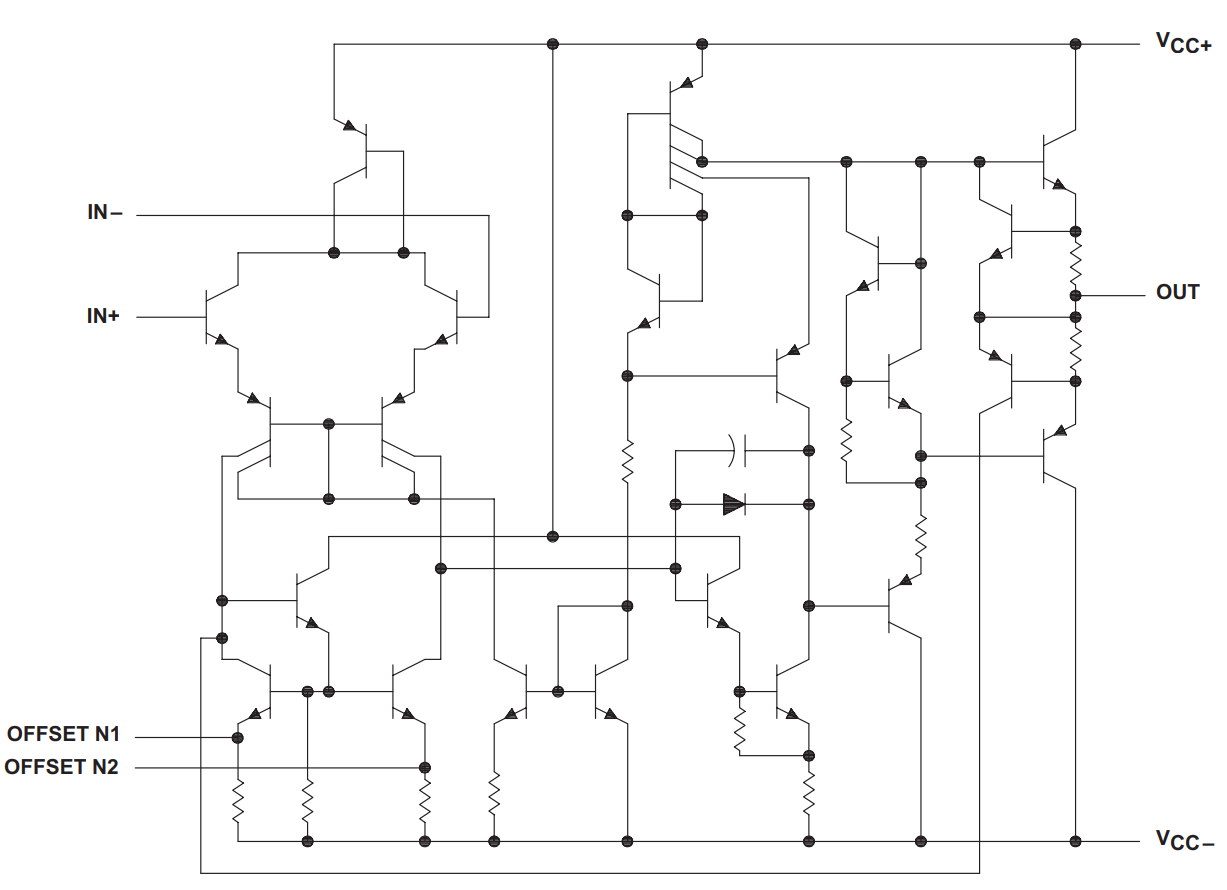
\includegraphics[width=0.5\linewidth]{芯片内部}
		\caption{芯片内部设计}
	\end{figure}	
	\begin{figure}[h]
		\begin{minipage}[t]{0.33\textwidth}
			\centering
			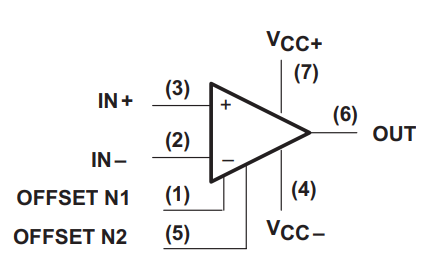
\includegraphics[width=0.9\linewidth]{简化内部}
			\caption{芯片示意图}
		\end{minipage}
		\begin{minipage}[t]{0.33\textwidth}
			\centering
			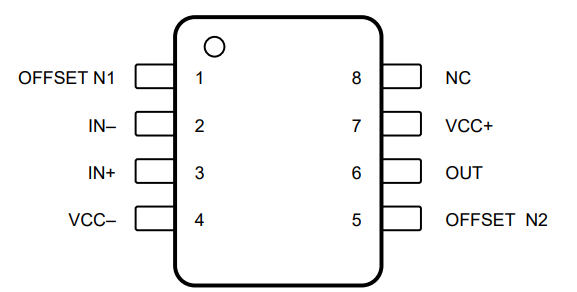
\includegraphics[width=0.9\linewidth]{引脚}
			\caption{芯片引脚}
		\end{minipage}
		\begin{minipage}[t]{0.33\textwidth}
			\centering
			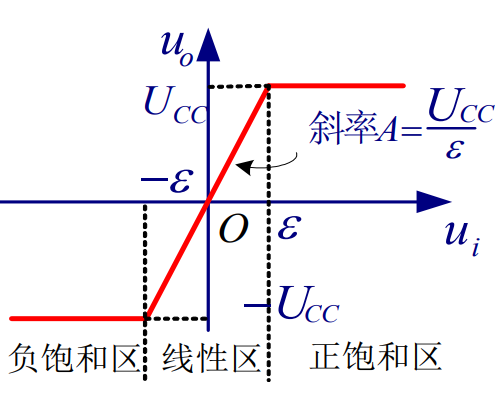
\includegraphics[width=0.7\linewidth]{图线}
			\caption{工作图线}
		\end{minipage}		
	\end{figure}

	在图示引脚中, 7端接入 +12V Vcc 直流电源, 4 接入 -12V -Vcc 直流电源. 2为反相输入端, 3为同相输入端，6为输出. 1和5为偏置(调零端), 8空脚, 通常悬空. 
	
	在电路中, 运算放大器通常具有"虚短"和"虚断"特性:
	\begin{itemize}
	\item 理想情况下, 流入集成运算放大器的输入端电流为0, 理想运放的输入电阻无限大, 近似认为运放的两个输入端开路. 
	\item 理想情况下, 近似认为两输入端电位相等.
	\item 特性成立条件: 运放的开环增益足够大(运放工作在线性区), 有反馈电路
	\end{itemize}
	
	利用以上功能和特性, 可以设计实现基本运算电路. 
	
	\section{实验过程与结果}
	使用DC电源产生串联的双12V直流电源为UA741芯片供电.
	
	\subsection{反相比例电路}
	如图所示的电路图完成线路连接. 需要计算电路中电阻的大小参数. 
	
	\begin{figure}[h]
		\centering
		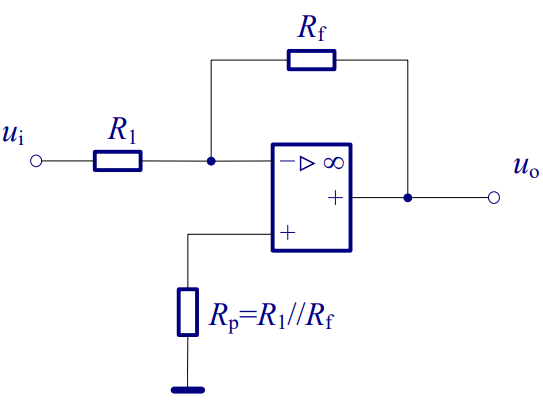
\includegraphics[width=0.3\linewidth]{反向电路图}
		\caption{反相放大器电路原理图}
	\end{figure}
	
	根据虚短和虚断的特性, 列写方程
	$$
	\left\{ 
	\begin{aligned}
		u_+&=u_-=0\\
		\frac{u_0-u_-}{R_f}&=-\frac{u_i-u_-}{R_1}
	\end{aligned}
	\right.
	$$
	可得$\frac{u_0}{R_f}=-\frac{u_i}{R_1}$. 使用参数$R_f=5k\Omega,~R_1=1k\Omega$, 计算出$R_p=\frac{5}{6}k\Omega$. 使用波形发生器产生1kHz/100mVpp的正弦波形作为输入. 使用示波器同时观察输入输出信号如图所示. 
	
	\begin{figure}[h]
		\begin{minipage}[t]{0.5\linewidth}
			\centering
			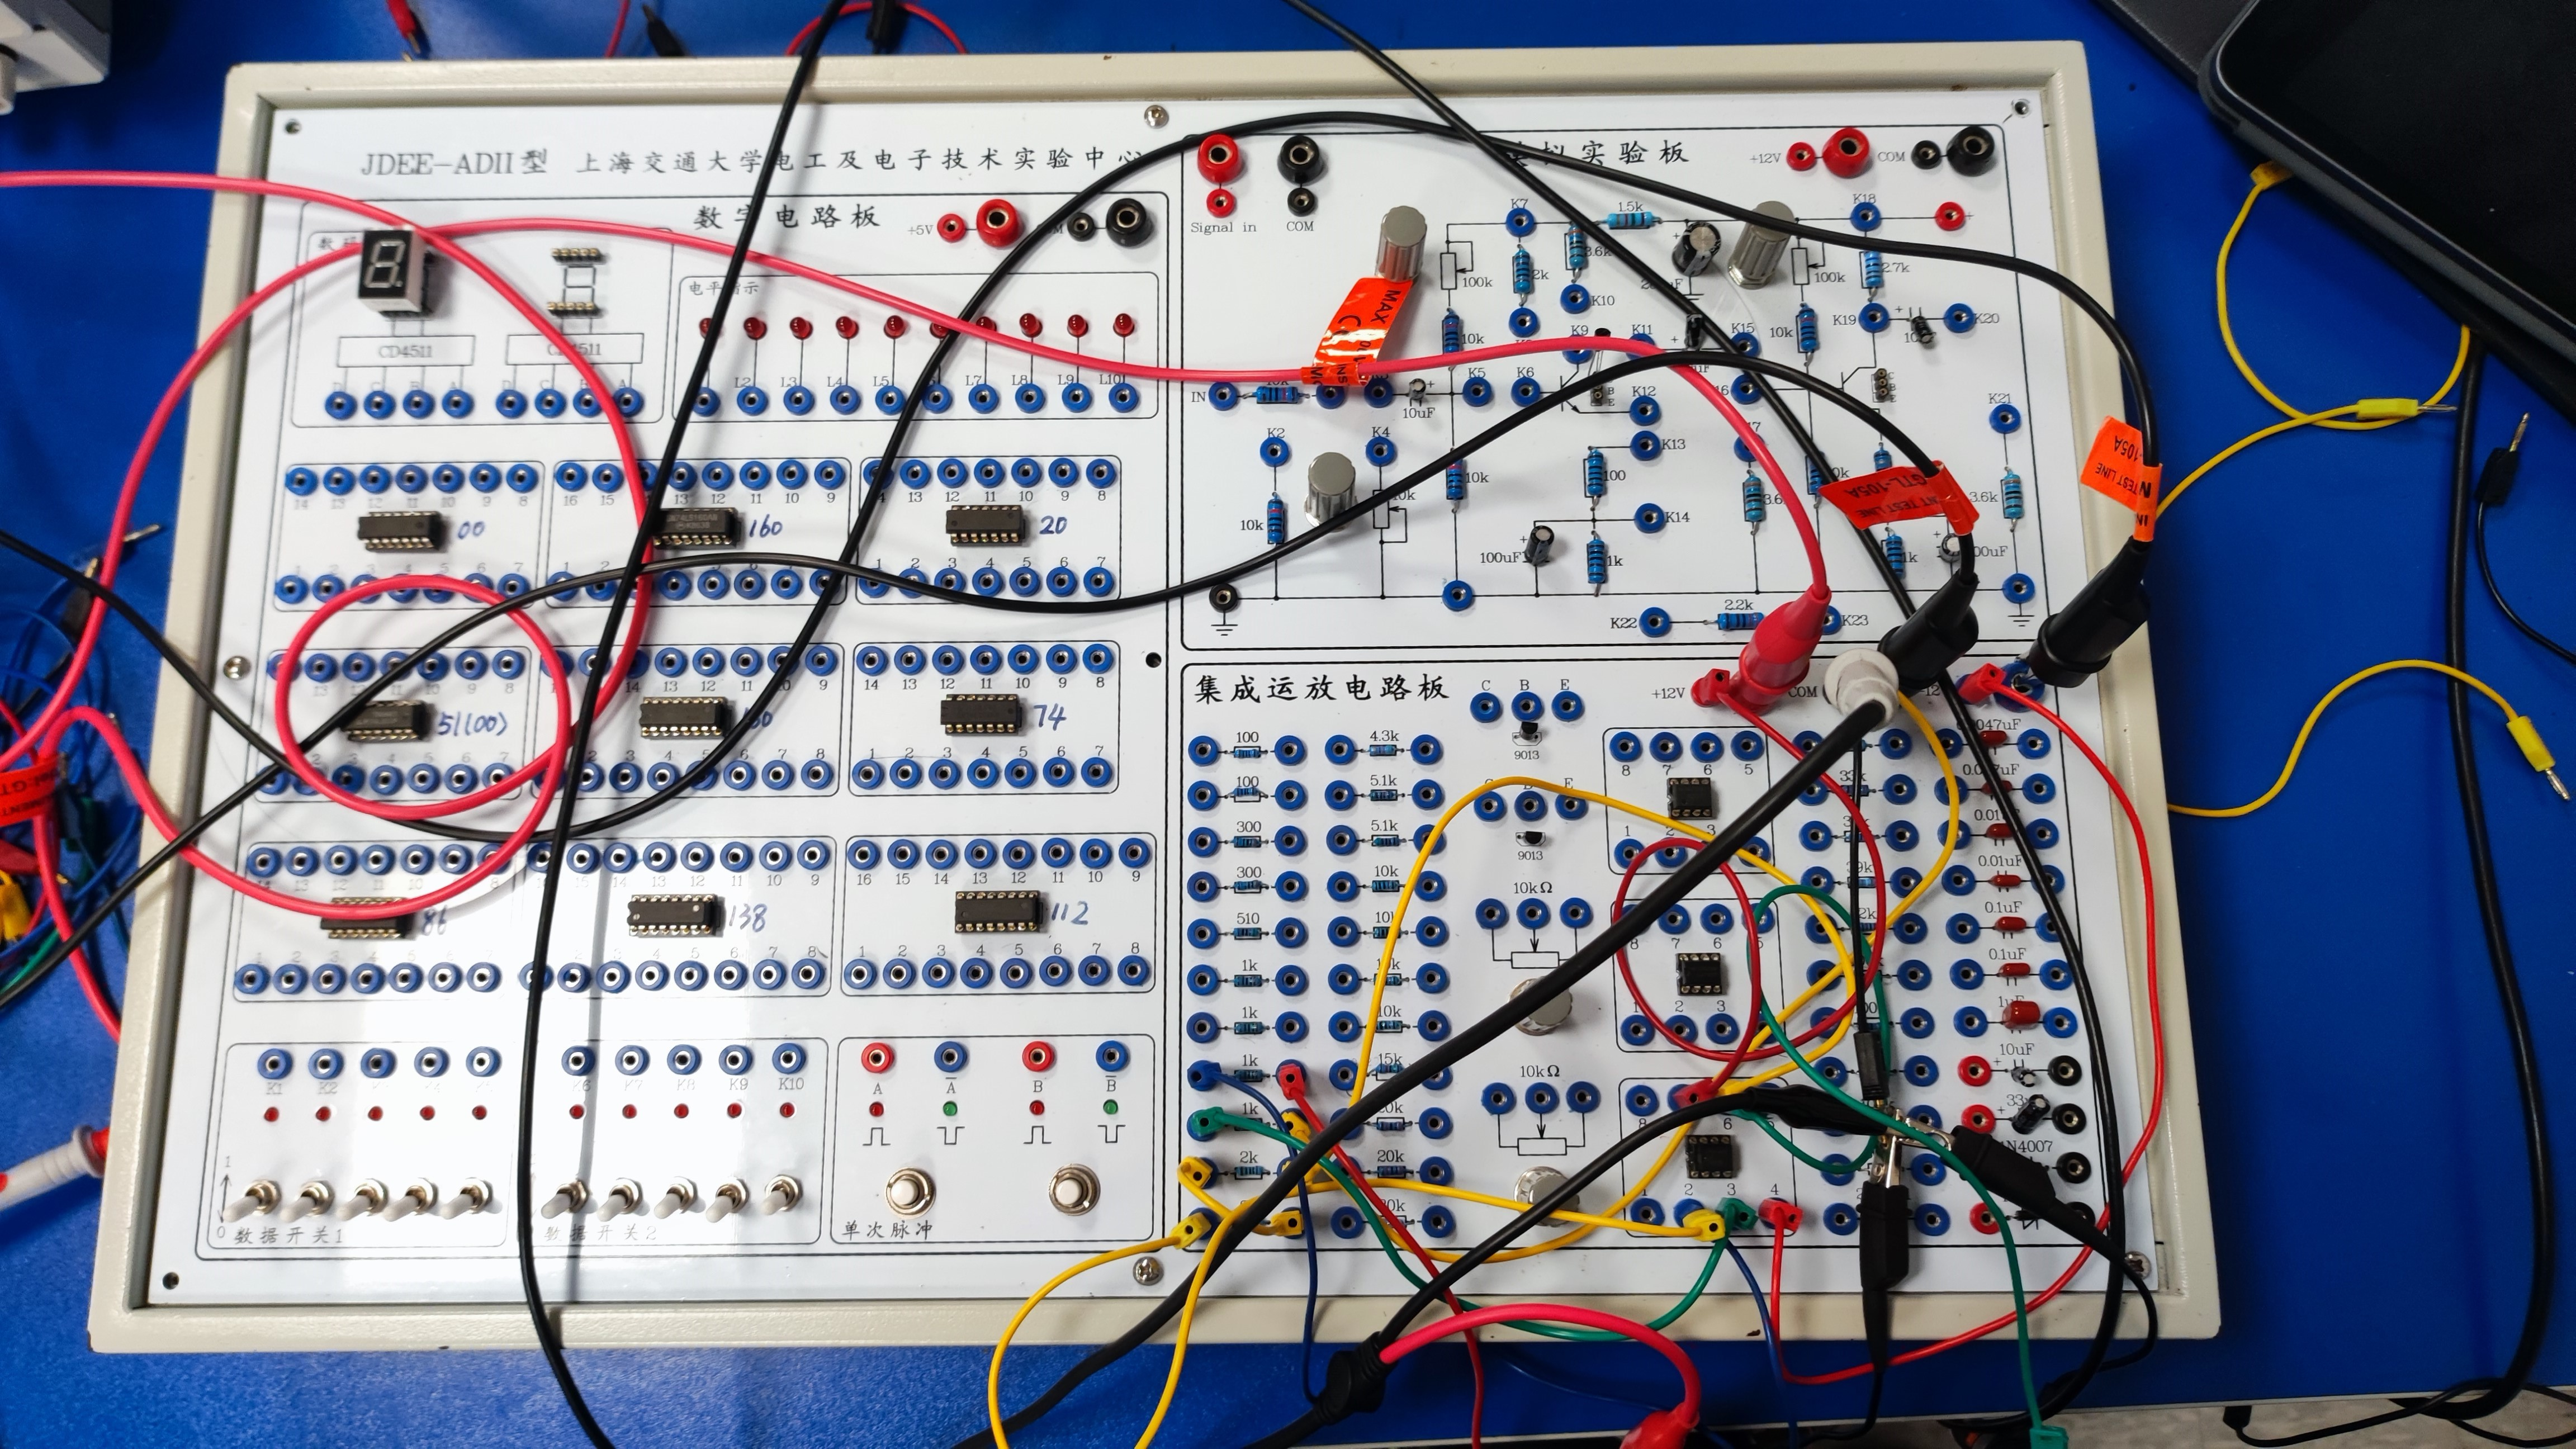
\includegraphics[width=0.9\linewidth]{../图片/反向放大器连线}
			\caption{反相放大器实物图}
		\end{minipage}
		\begin{minipage}[t]{0.5\linewidth}
			\centering
			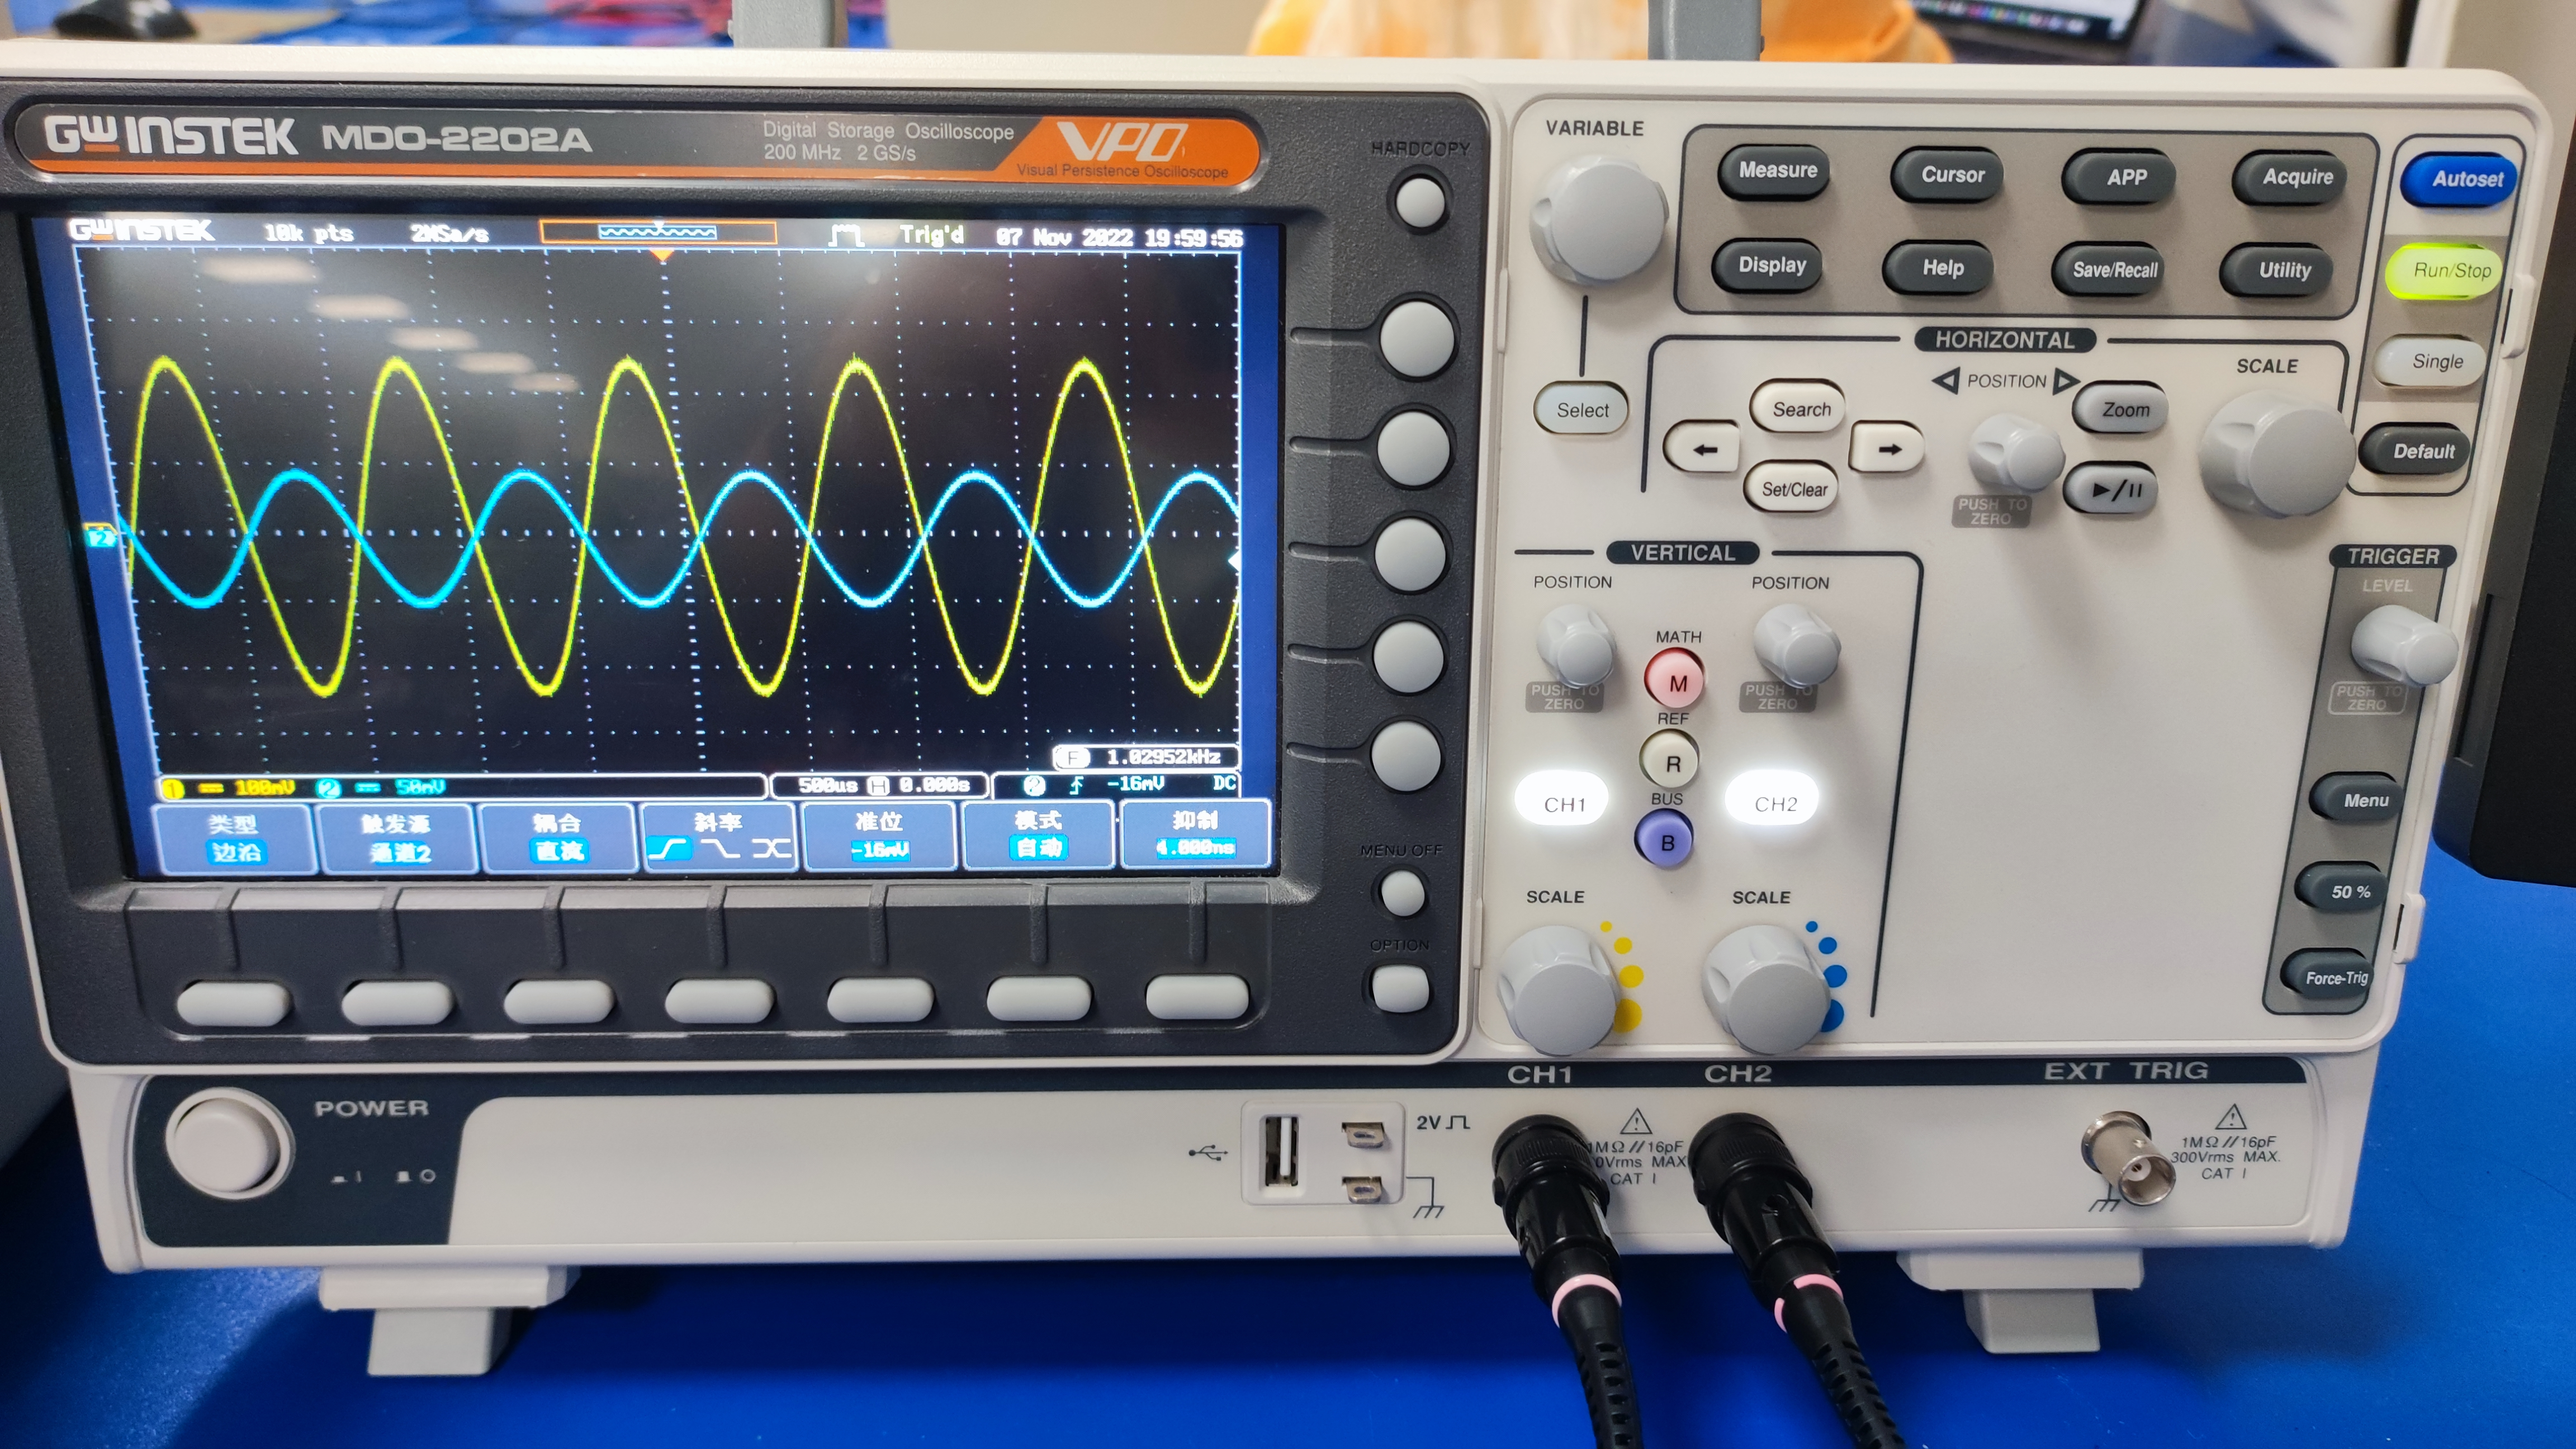
\includegraphics[width=0.9\linewidth]{../图片/反向放大器示波器}
			\caption{反相放大器示波器图线}
		\end{minipage}		
	\end{figure}

	发现输入输出信号都是1kHZ的正弦波, 其中输入信号为100mVpp, 输出信号与输入信号反相且幅值为500mVpp. 基本符合预期结果. 
	
	反相放大电路是使用运算放大器实现的最基本的基本运算电路, 可用于检测芯片功能是否完好. 
	
	\subsection{反相加法器}
	如图所示连接电路. 
	
	\begin{figure}[h]
		\begin{minipage}[t]{0.5\linewidth}
			\centering
			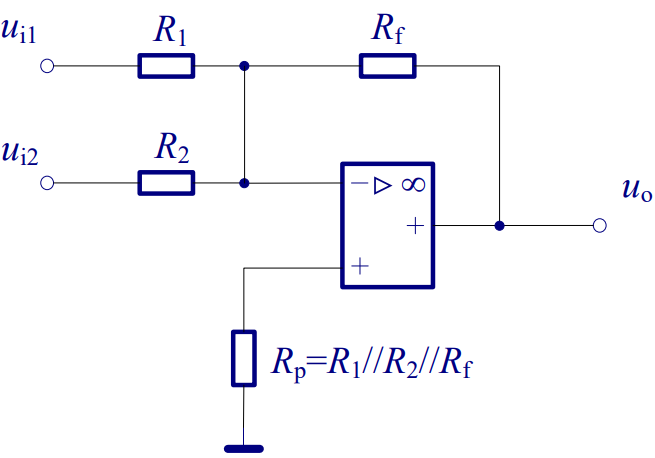
\includegraphics[width=0.7\linewidth]{加法器原理图}
			\caption{加法器原理图}
		\end{minipage}
		\begin{minipage}[t]{0.5\linewidth}
			\centering
			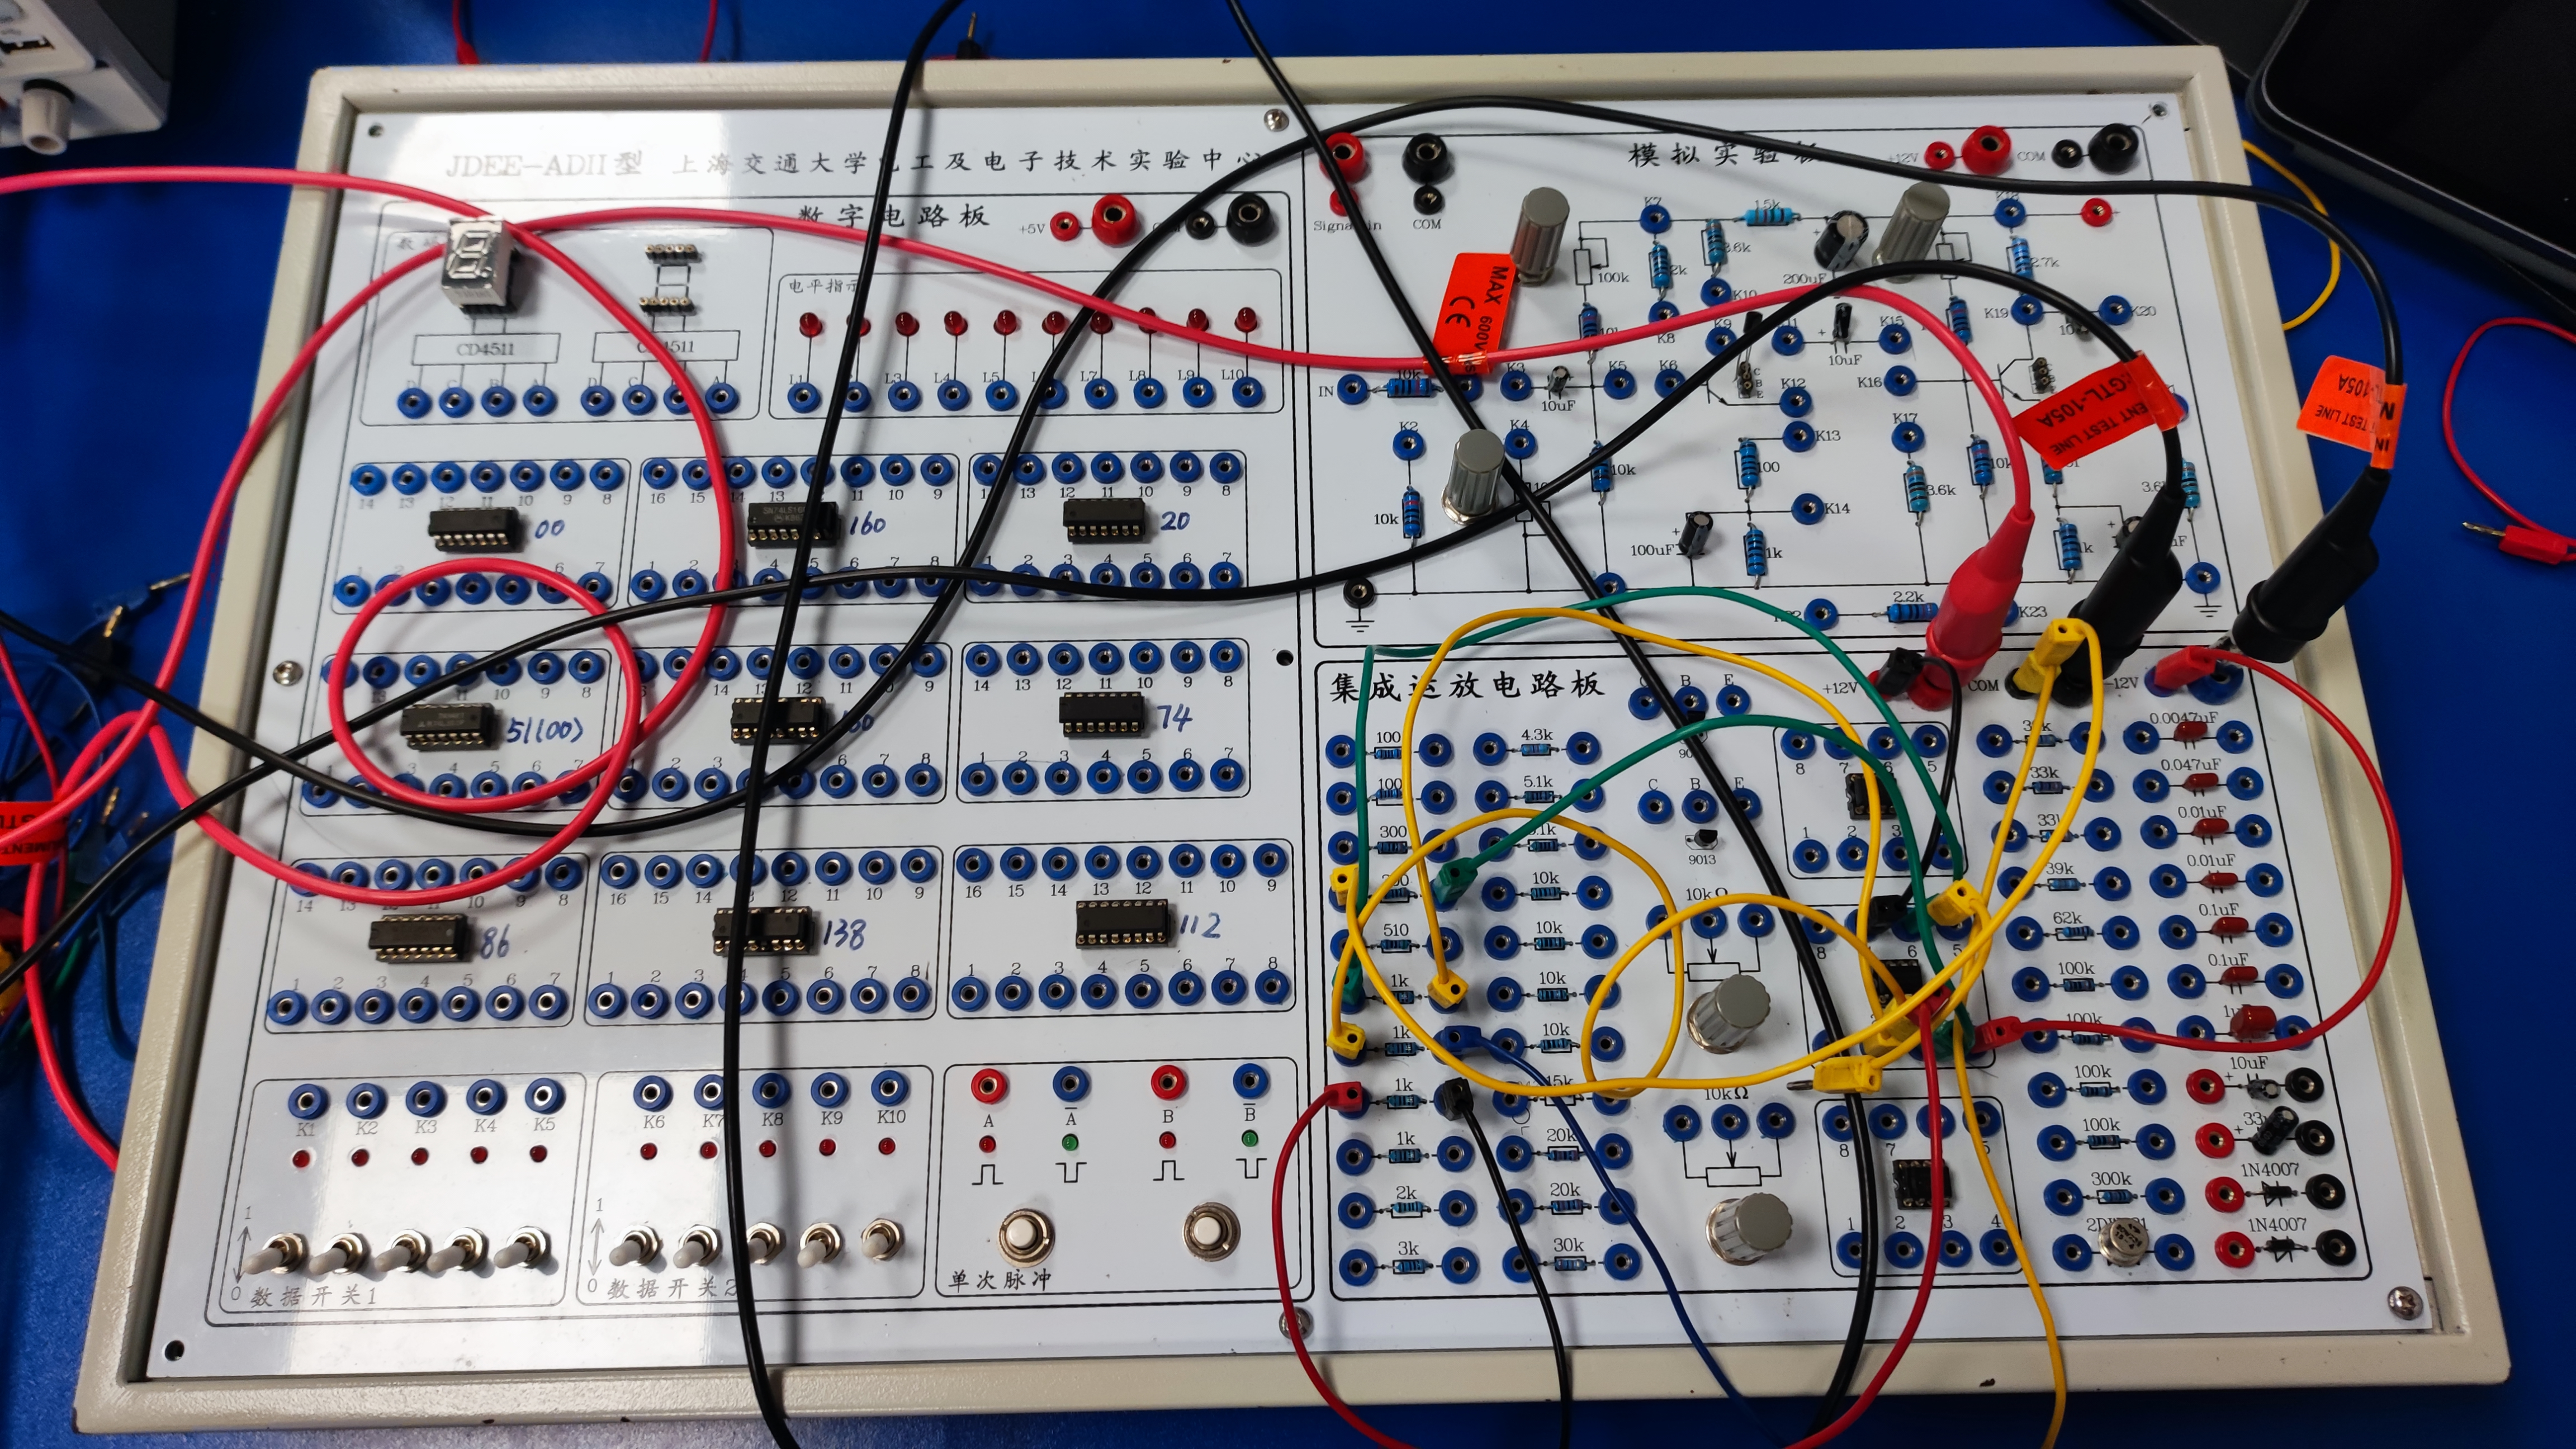
\includegraphics[width=0.9\linewidth]{../图片/加法器连线}
			\caption{加法器实物图}
		\end{minipage}		
	\end{figure}

	根据电路图和所需实现的功能列写方程
	$$
	\left\{ 
	\begin{aligned}
		u_+=u_-&=0\\
		\frac{u_1-u_-}{R_1}+\frac{u_2-u_-}{R_2}&=-\frac{u_o-u_-}{R_f}
	\end{aligned}
	\right.
	$$
	即$\frac{u_1}{R_1}+\frac{u_2}{R_2}=-\frac{u_o}{R_f}$. 根据加法器所需功能, 应有$R_1=R_2=R$. 故$u_1+u_2=-\frac{u_o\cdot R}{R_f}$. 选取参数$R=R_f=1k\Omega$并使用相应的$R_p$, 有$u_1+u_2=-u_o$, 如图所示的示波器图线显示了输入与输出间的关系. 
	
	\begin{figure}[h]
		\begin{minipage}[t]{0.5\linewidth}
			\centering
			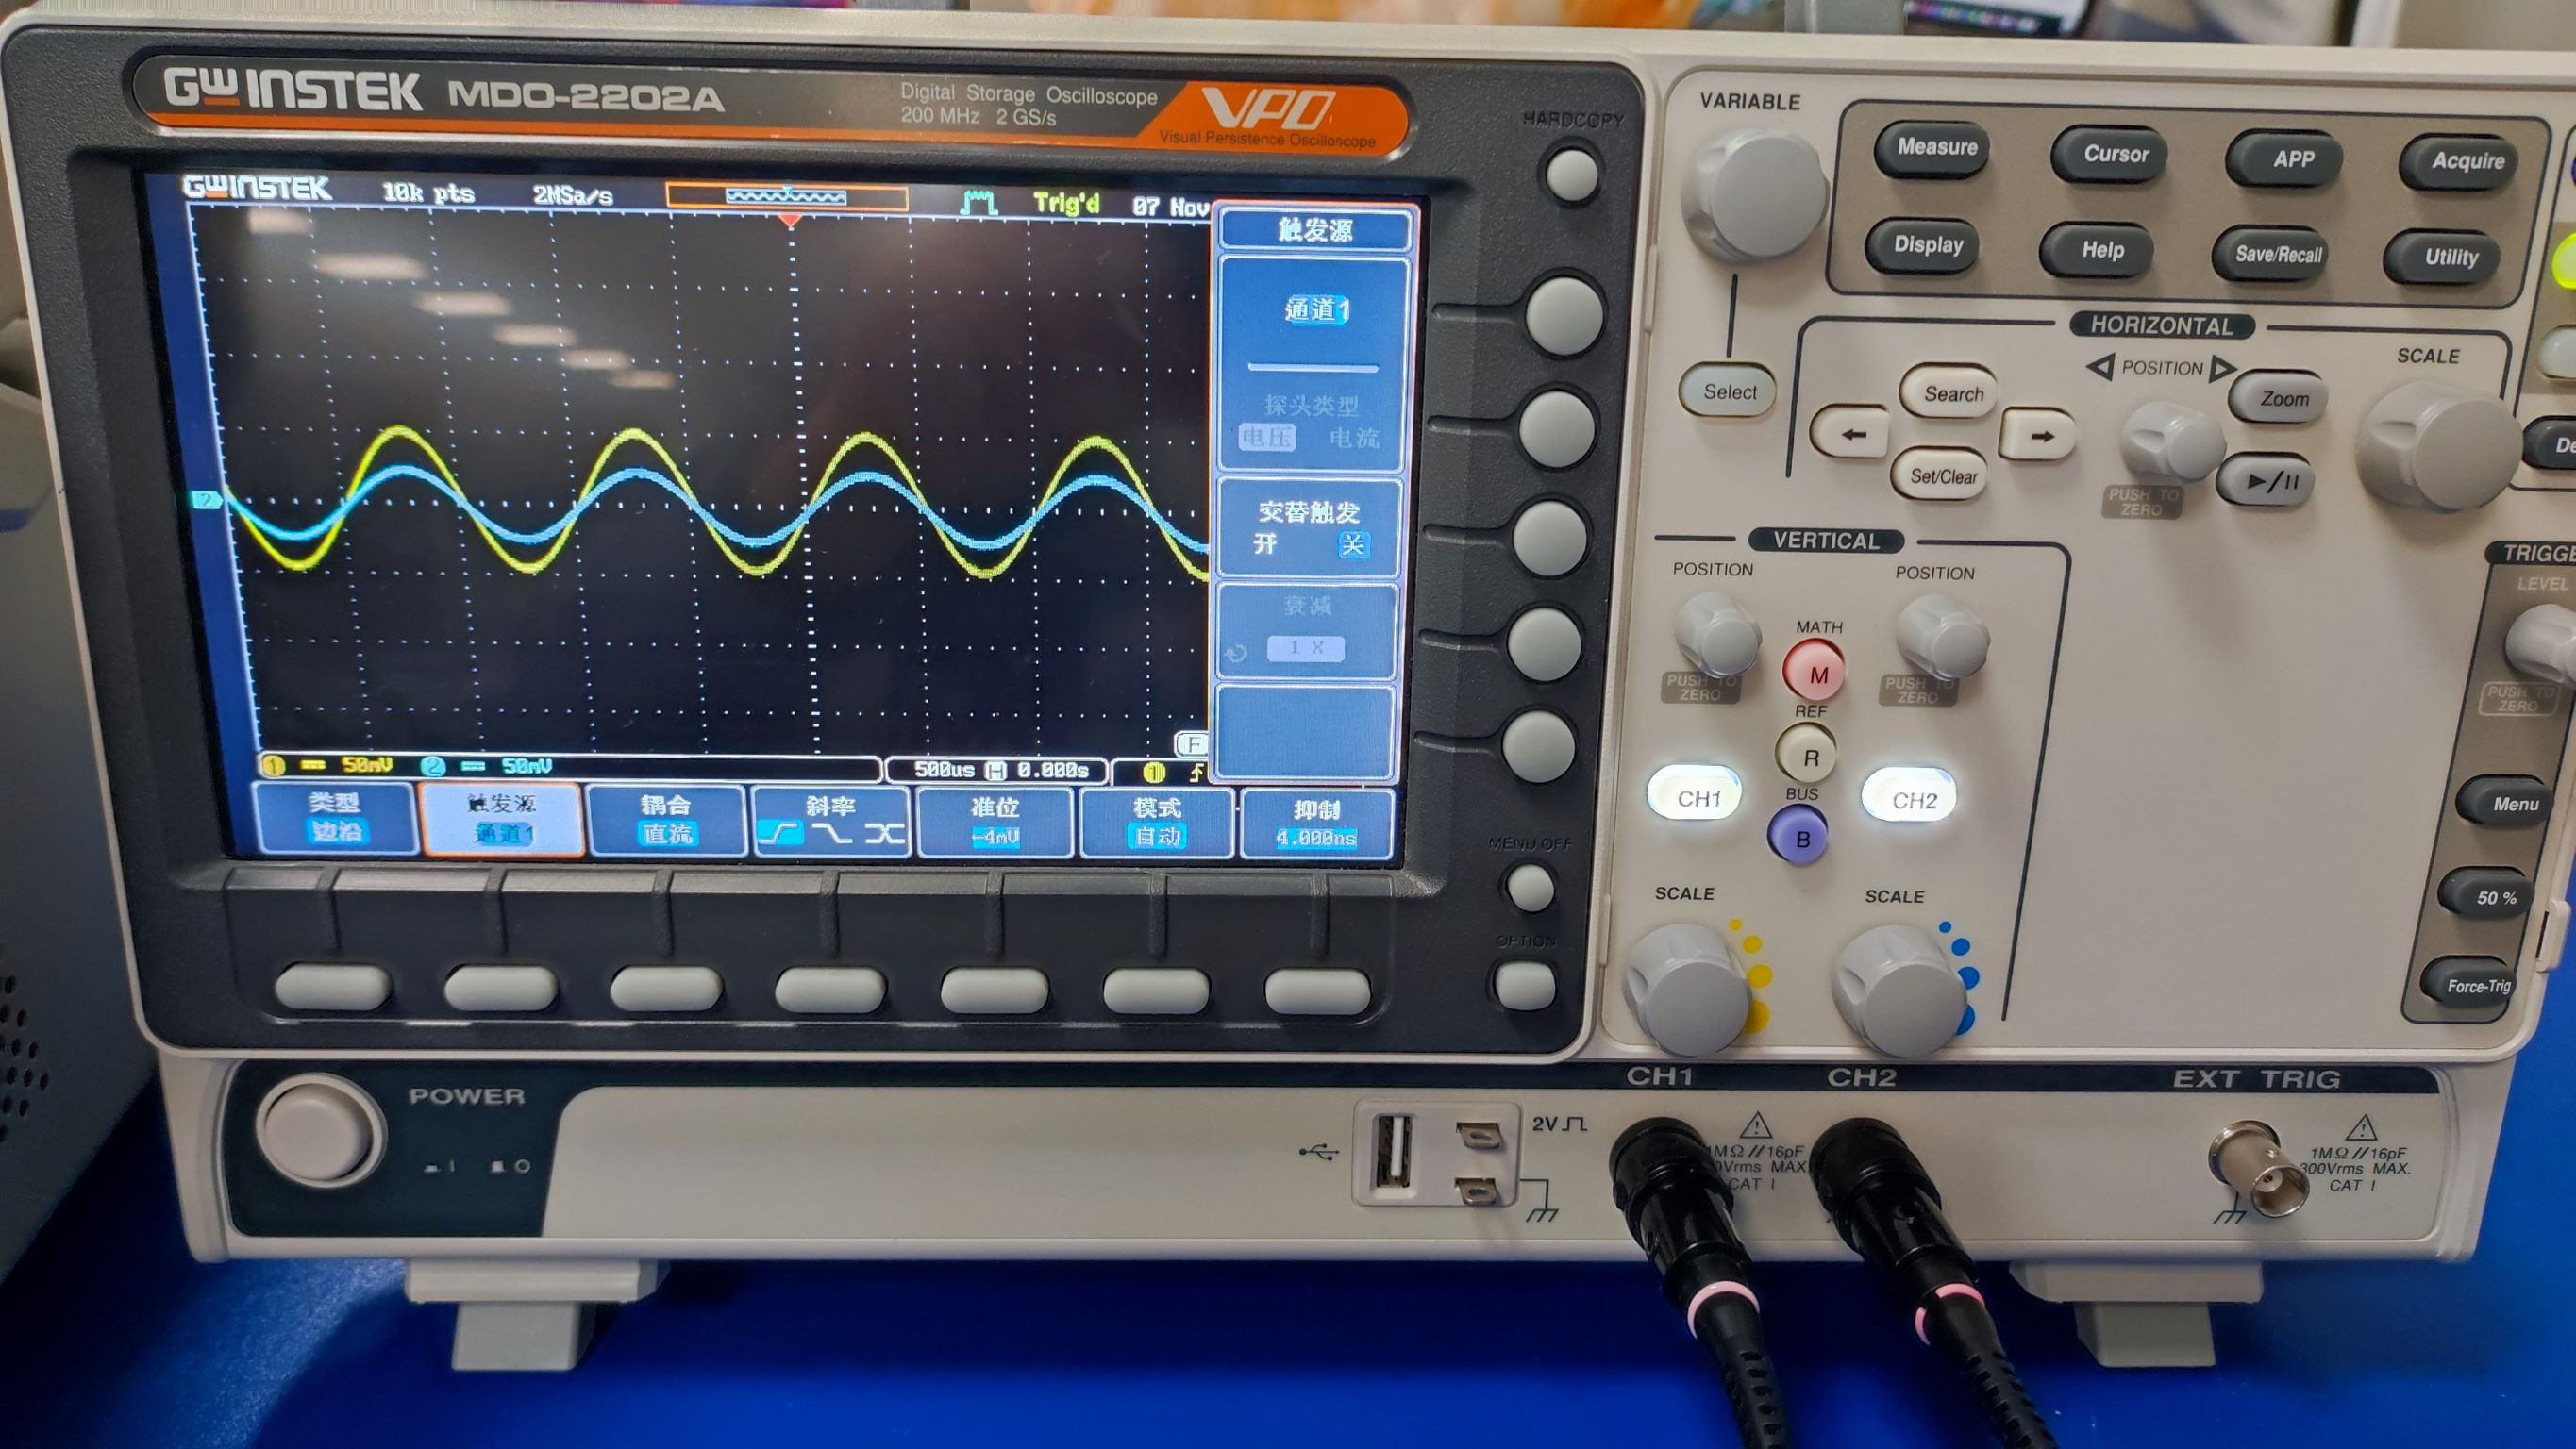
\includegraphics[width=0.9\linewidth]{../图片/加法器输入}
			\caption{加法器示波器双输入}
		\end{minipage}
		\begin{minipage}[t]{0.5\linewidth}
			\centering
			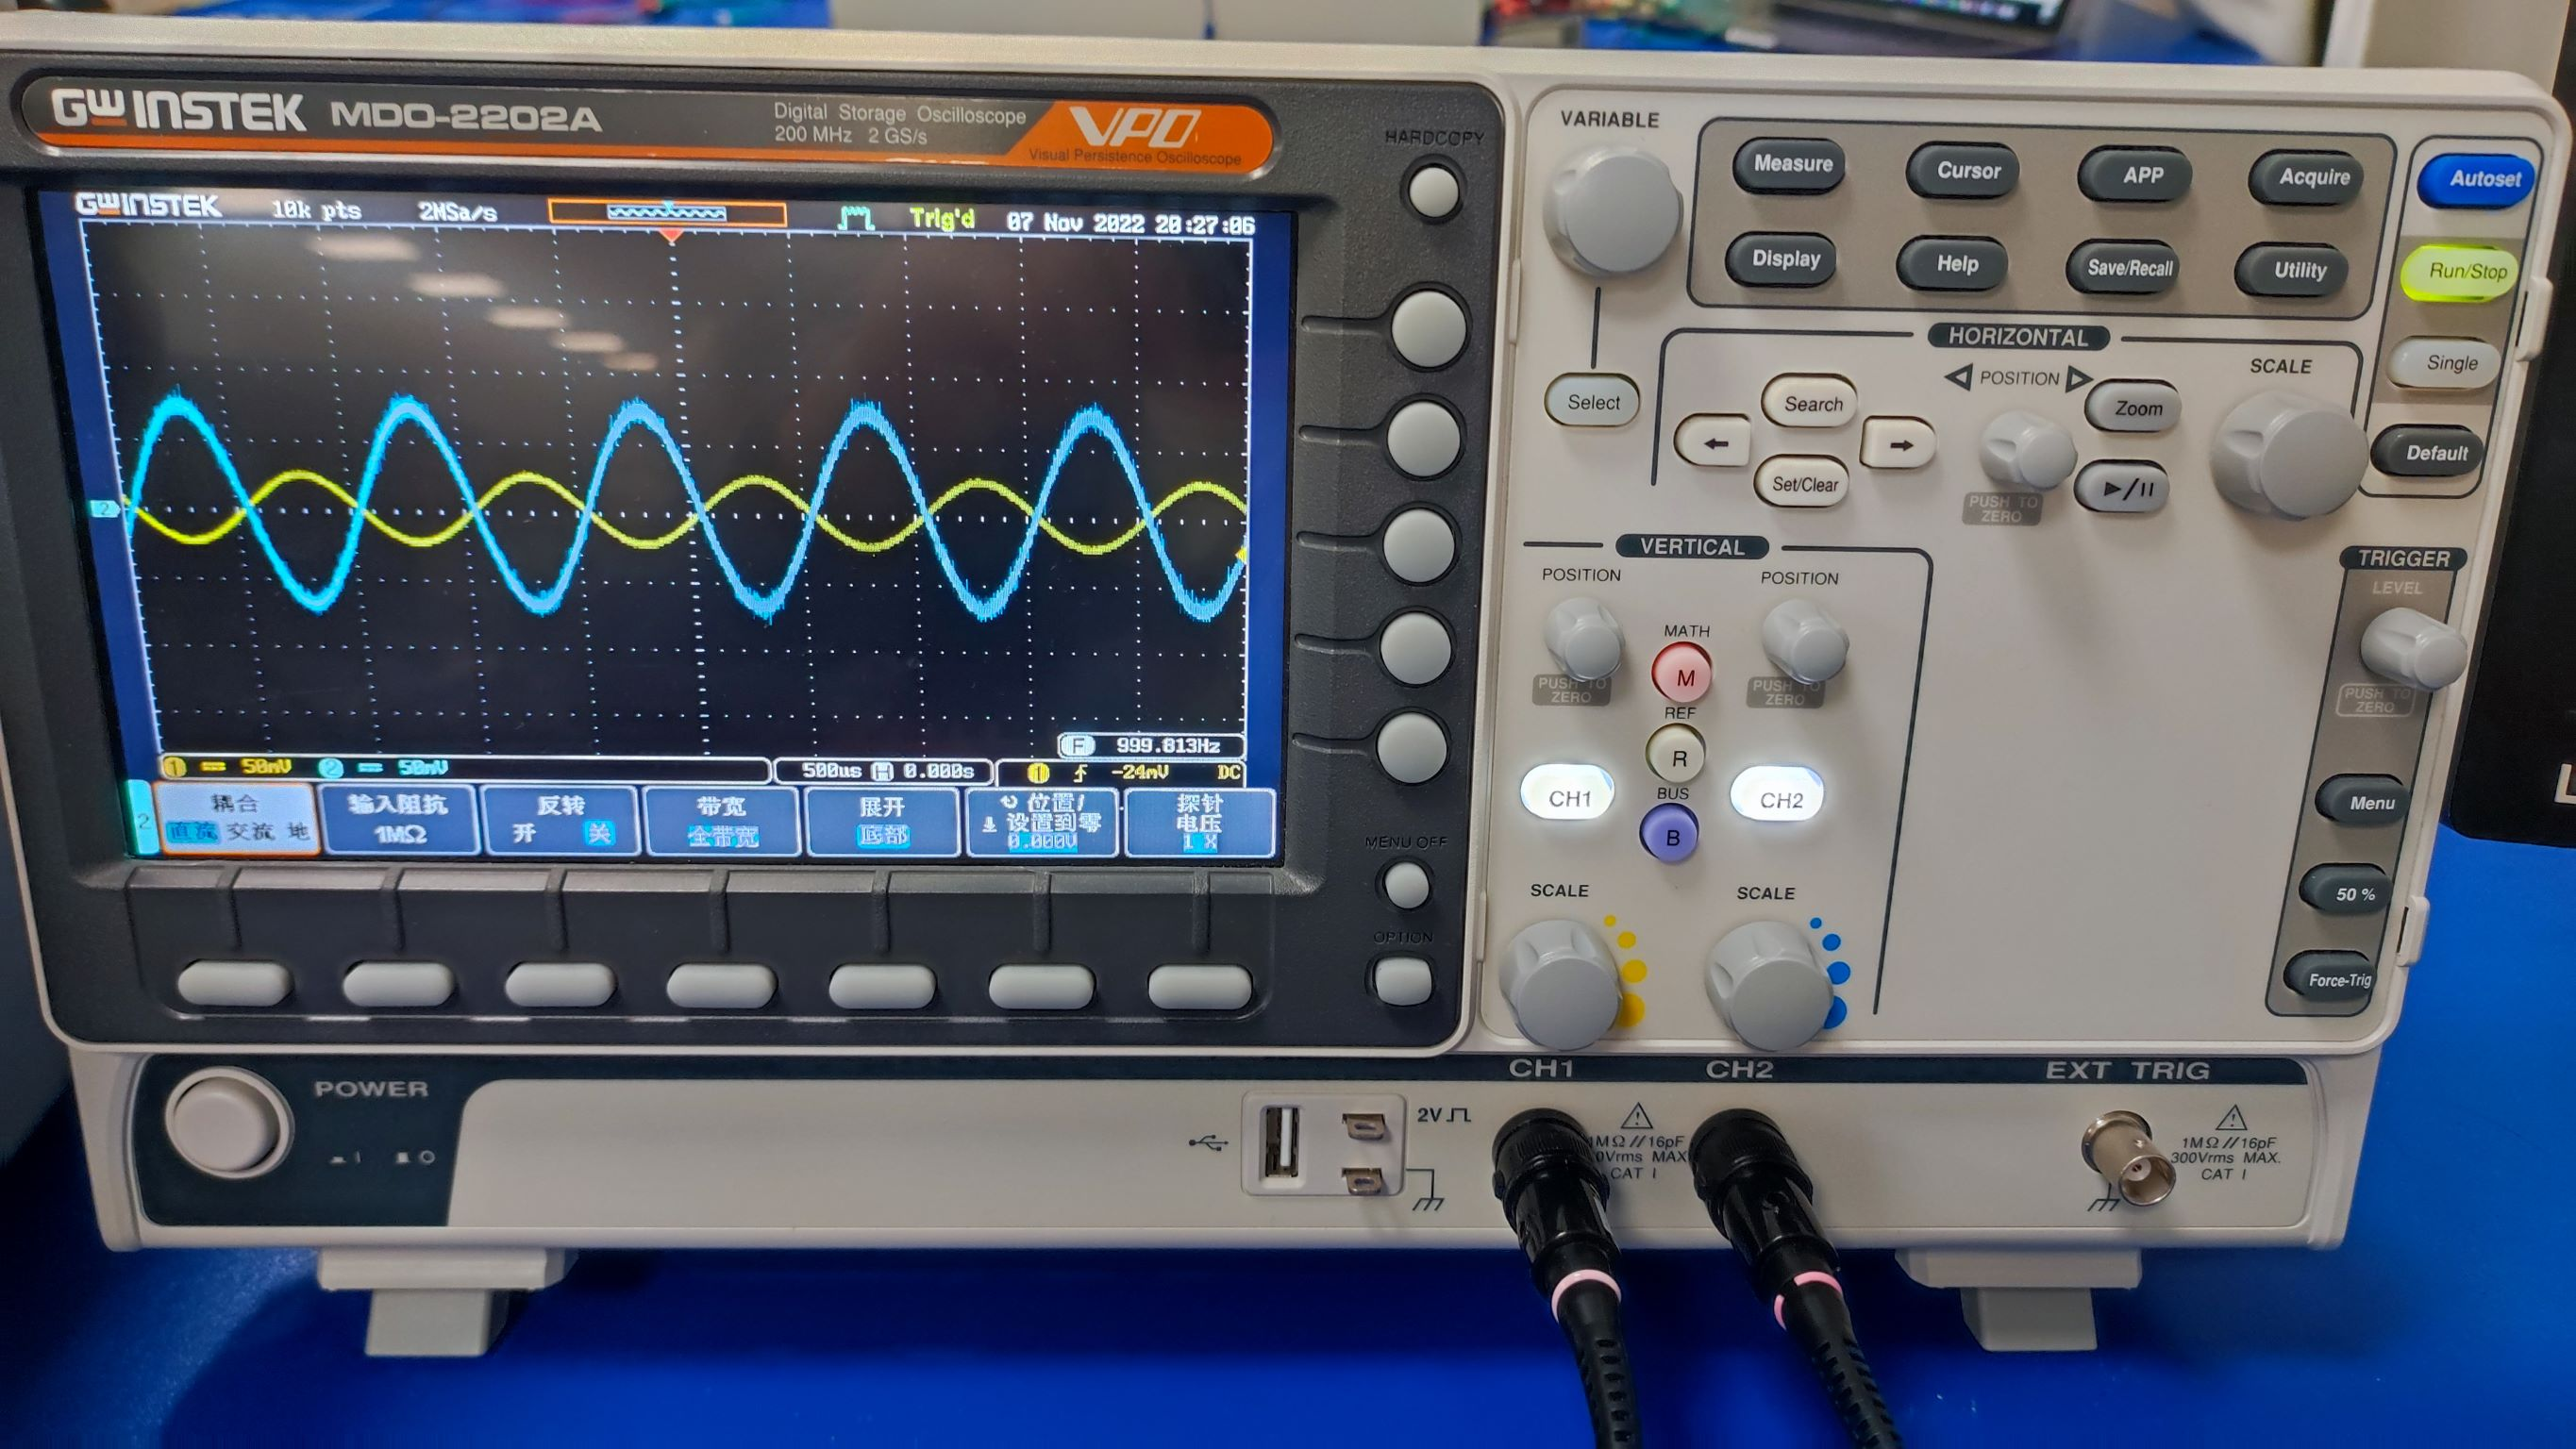
\includegraphics[width=0.9\linewidth]{../图片/加法器输入输出}
			\caption{加法器示波器输入和输出}
		\end{minipage}		
	\end{figure}

	输入为1kHz/100mVpp的正弦和1kHz/50mVpp的同相正弦. 第一种图中显示了两个输入波形. 第二张图显示了1kHz/50mVpp的正弦输入和输出波形, 发现两者都是1kHz的正弦波. 输出与输入反相, 且存在输出峰值大小为两输入峰值大小之和的关系.
	
	如需使$u_o=-2\cdot(u_1+u_2)$, 只需使用$2k\Omega$作为$R_f$即可, 原理与现象完全一致, 峰值变为两倍. 反相比例操作将在减法器中实现. 
	
	\subsection{反相比例减法器}
	电路原理图与实物图如图所示. 
	
	\begin{figure}[h]
		\begin{minipage}[t]{0.5\linewidth}
			\centering
			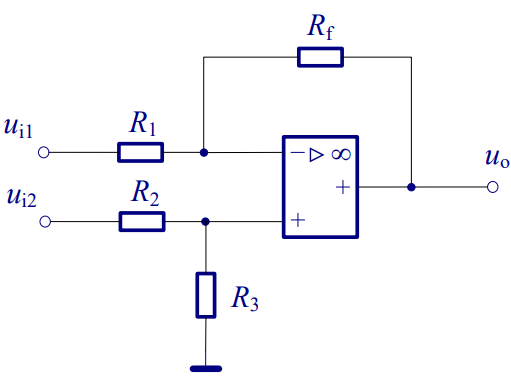
\includegraphics[width=0.7\linewidth]{减法器原理图}
			\caption{减法器原理图}
		\end{minipage}
		\begin{minipage}[t]{0.5\linewidth}
			\centering
			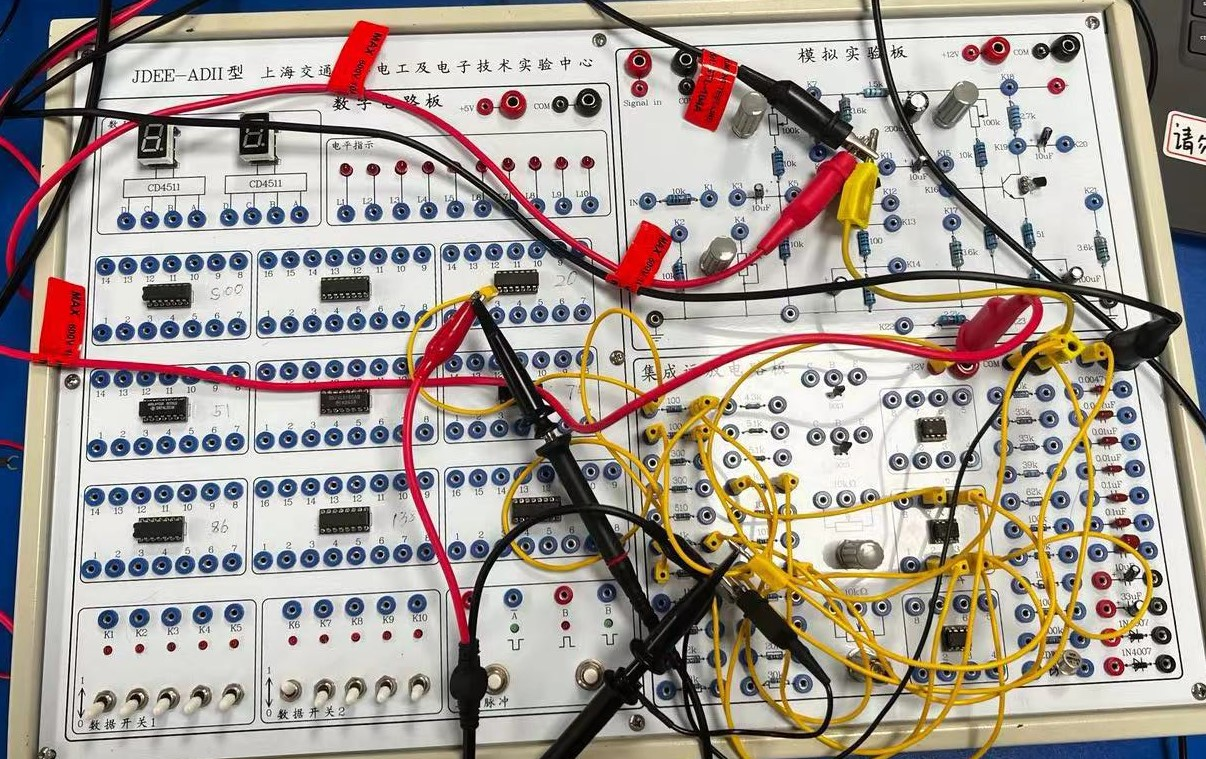
\includegraphics[width=0.9\linewidth]{../图片/减法器连线}
			\caption{减法器实物图}
		\end{minipage}		
	\end{figure}

	列写方程
	$$
	\left\{ 
	\begin{aligned}
		u_+=u_-&=\frac{u_{i2}\cdot R_3}{R_2+R_3}\\
		\frac{u_{i1}-u_-}{R_1}&=-\frac{u_o-u_-}{R_f}
	\end{aligned}
	\right.
	$$
	使用参数$R1=R2=1k\Omega, R_f=10k\Omega$. 为使$u_+$近似等于$u_{i2}$, 使用$R_3=300k\Omega$. 此时近似有$u_o=-10\cdot(u_{i1}-u_{i2})$. 示波器图线如图. 
	
	\begin{figure}[h]
		\begin{minipage}[t]{0.5\linewidth}
			\centering
			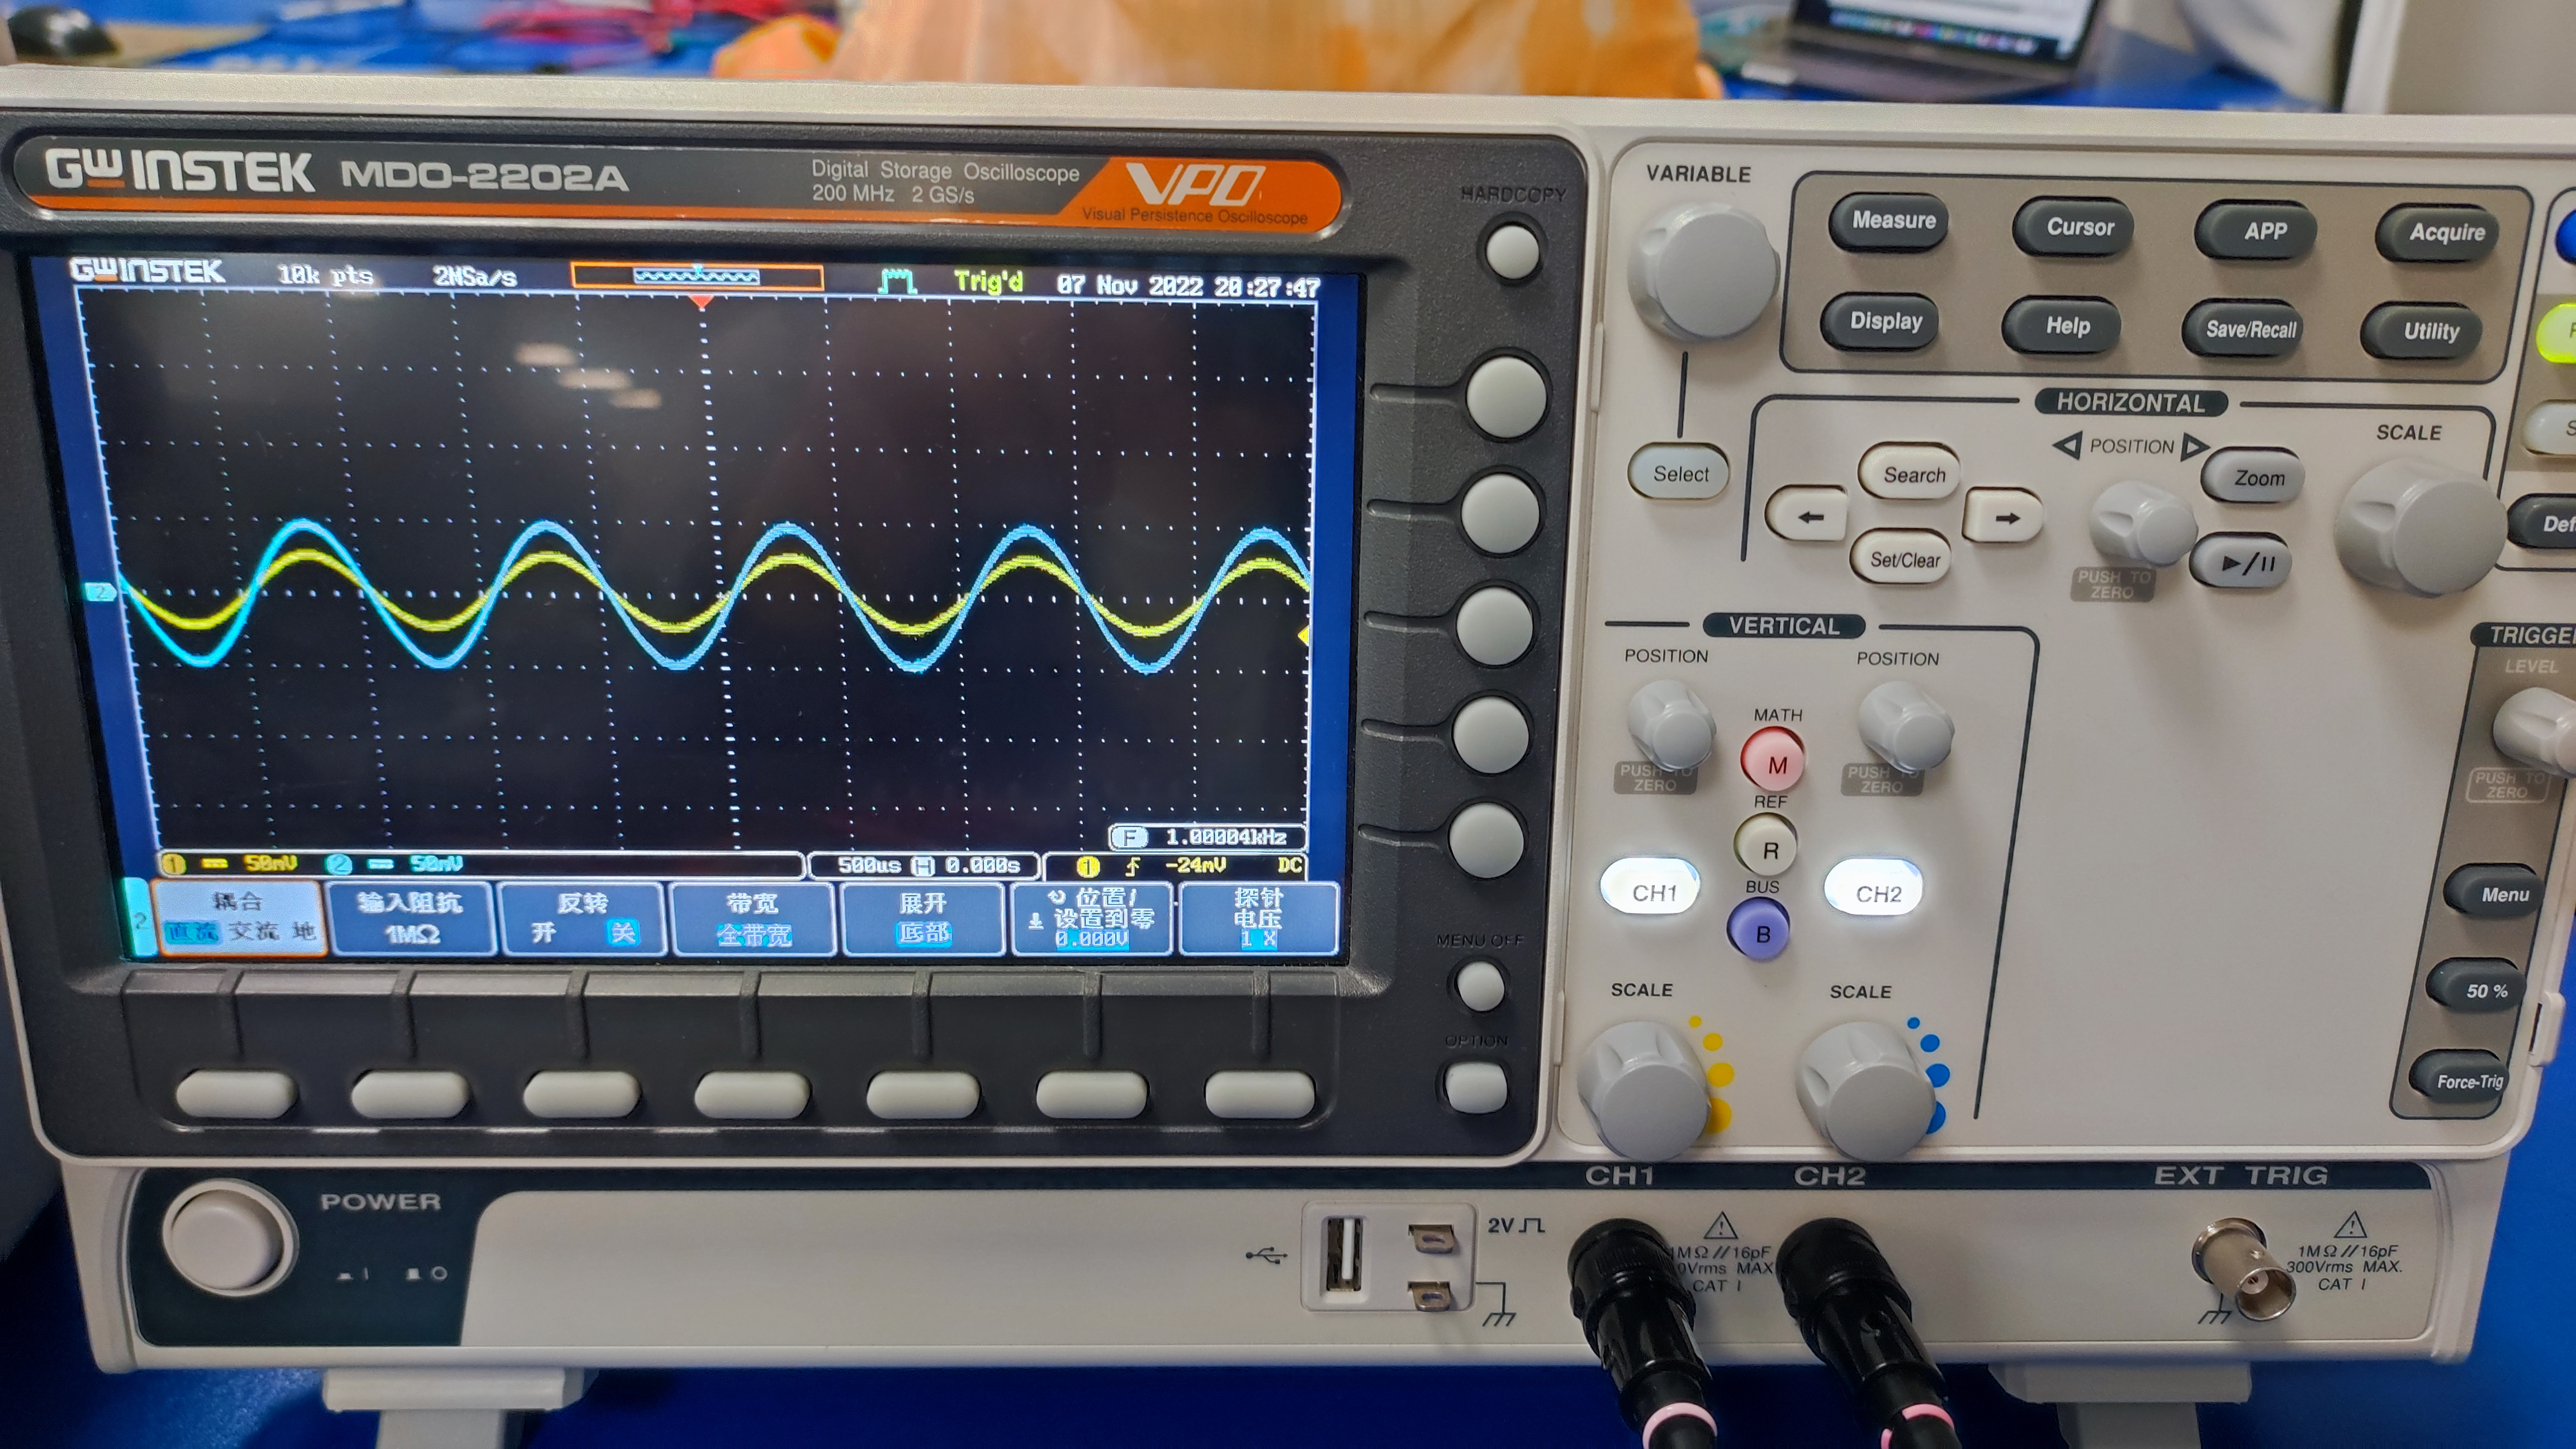
\includegraphics[width=0.9\linewidth]{../图片/减法器输入2}
			\caption{减法器示波器双输入}
		\end{minipage}
		\begin{minipage}[t]{0.5\linewidth}
			\centering
			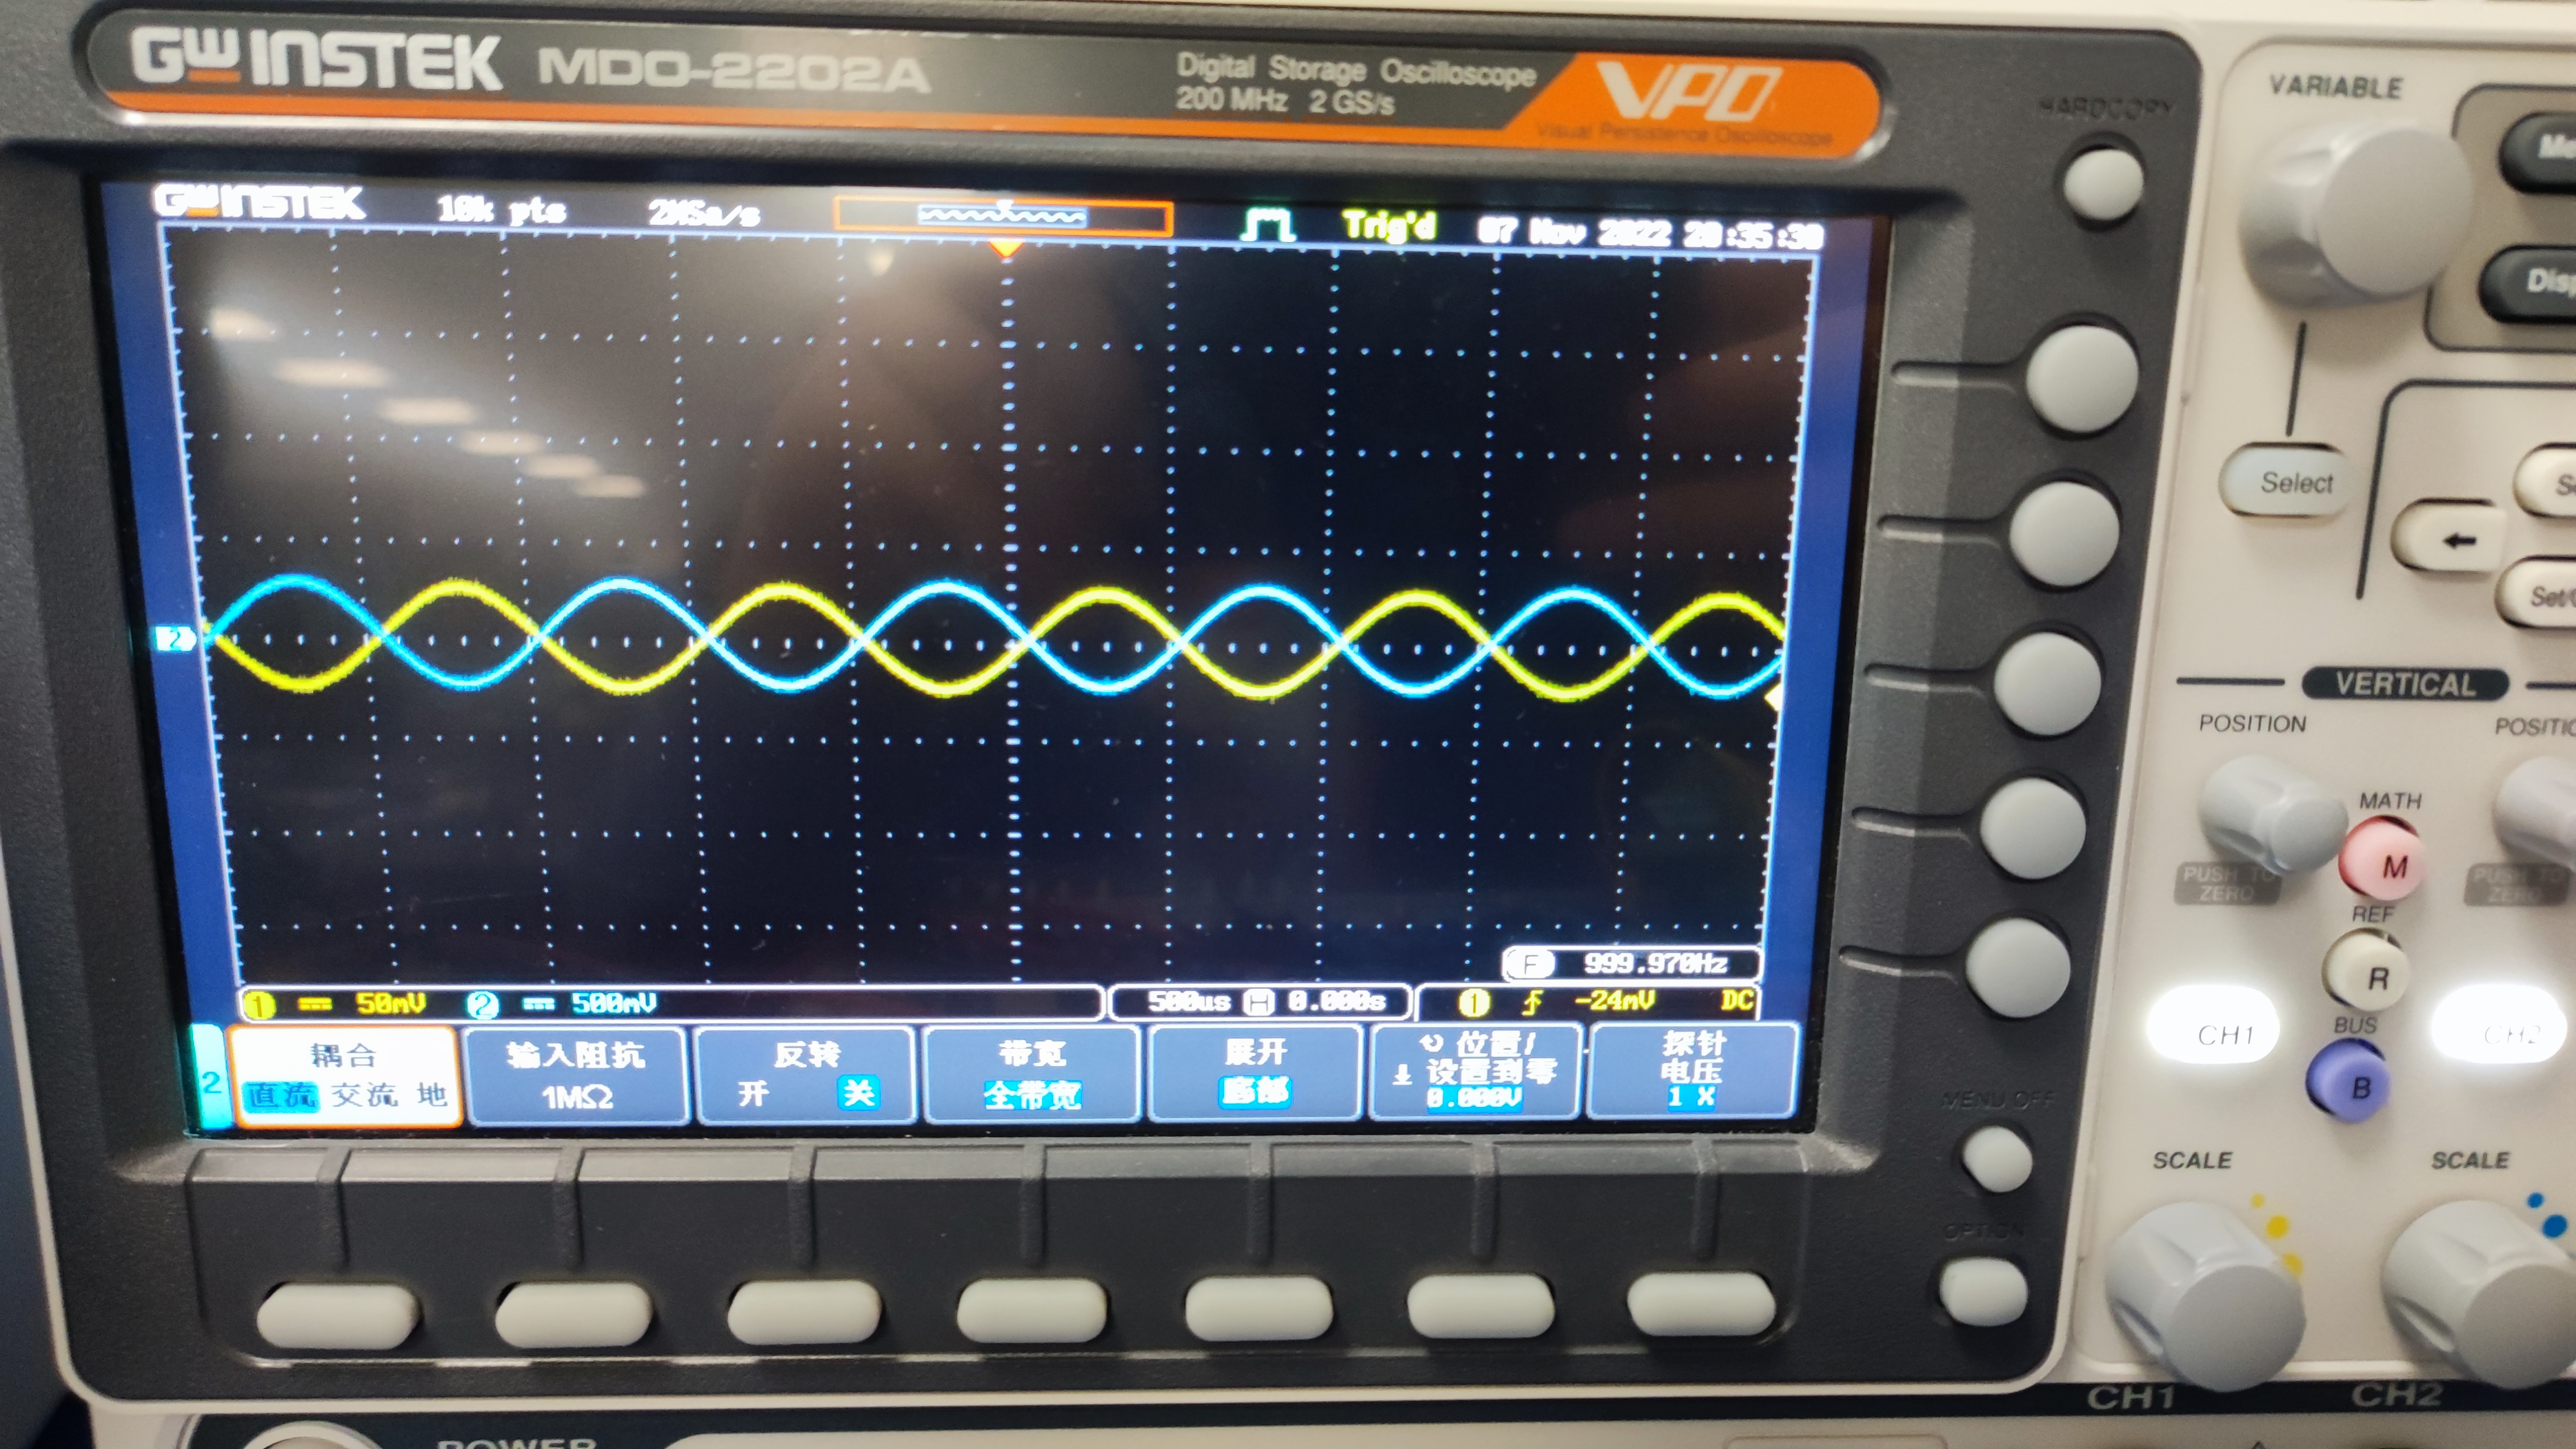
\includegraphics[width=0.9\linewidth]{../图片/减法器输入输出2}
			\caption{减法器示波器输入和输出}
		\end{minipage}		
	\end{figure}

	输出使用电桥实现同相不同Vpp. 示波器显示输入为1kHz的50mVpp和100mVpp的正弦波. 输出与输入反相, 且Vpp为输入两信号Vpp之差的10倍, 为500mVpp. 
	
	\subsection{积分器}
	积分器连接线路如图所示, 其中$R_f$处并联一开关, 用于观察去掉$R_f$的现象. 
	
	\begin{figure}[h]
		\begin{minipage}[t]{0.5\linewidth}
			\centering
			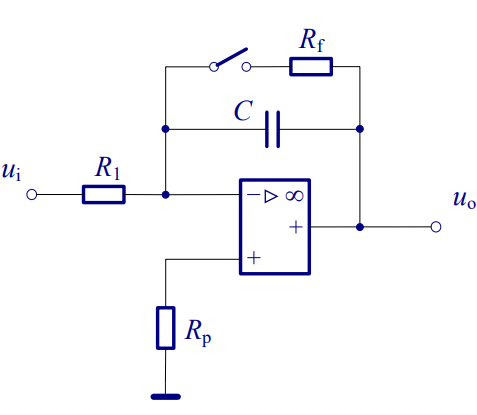
\includegraphics[width=0.6\linewidth]{积分器原理}
			\caption{积分器原理图}
		\end{minipage}
		\begin{minipage}[t]{0.5\linewidth}
			\centering
			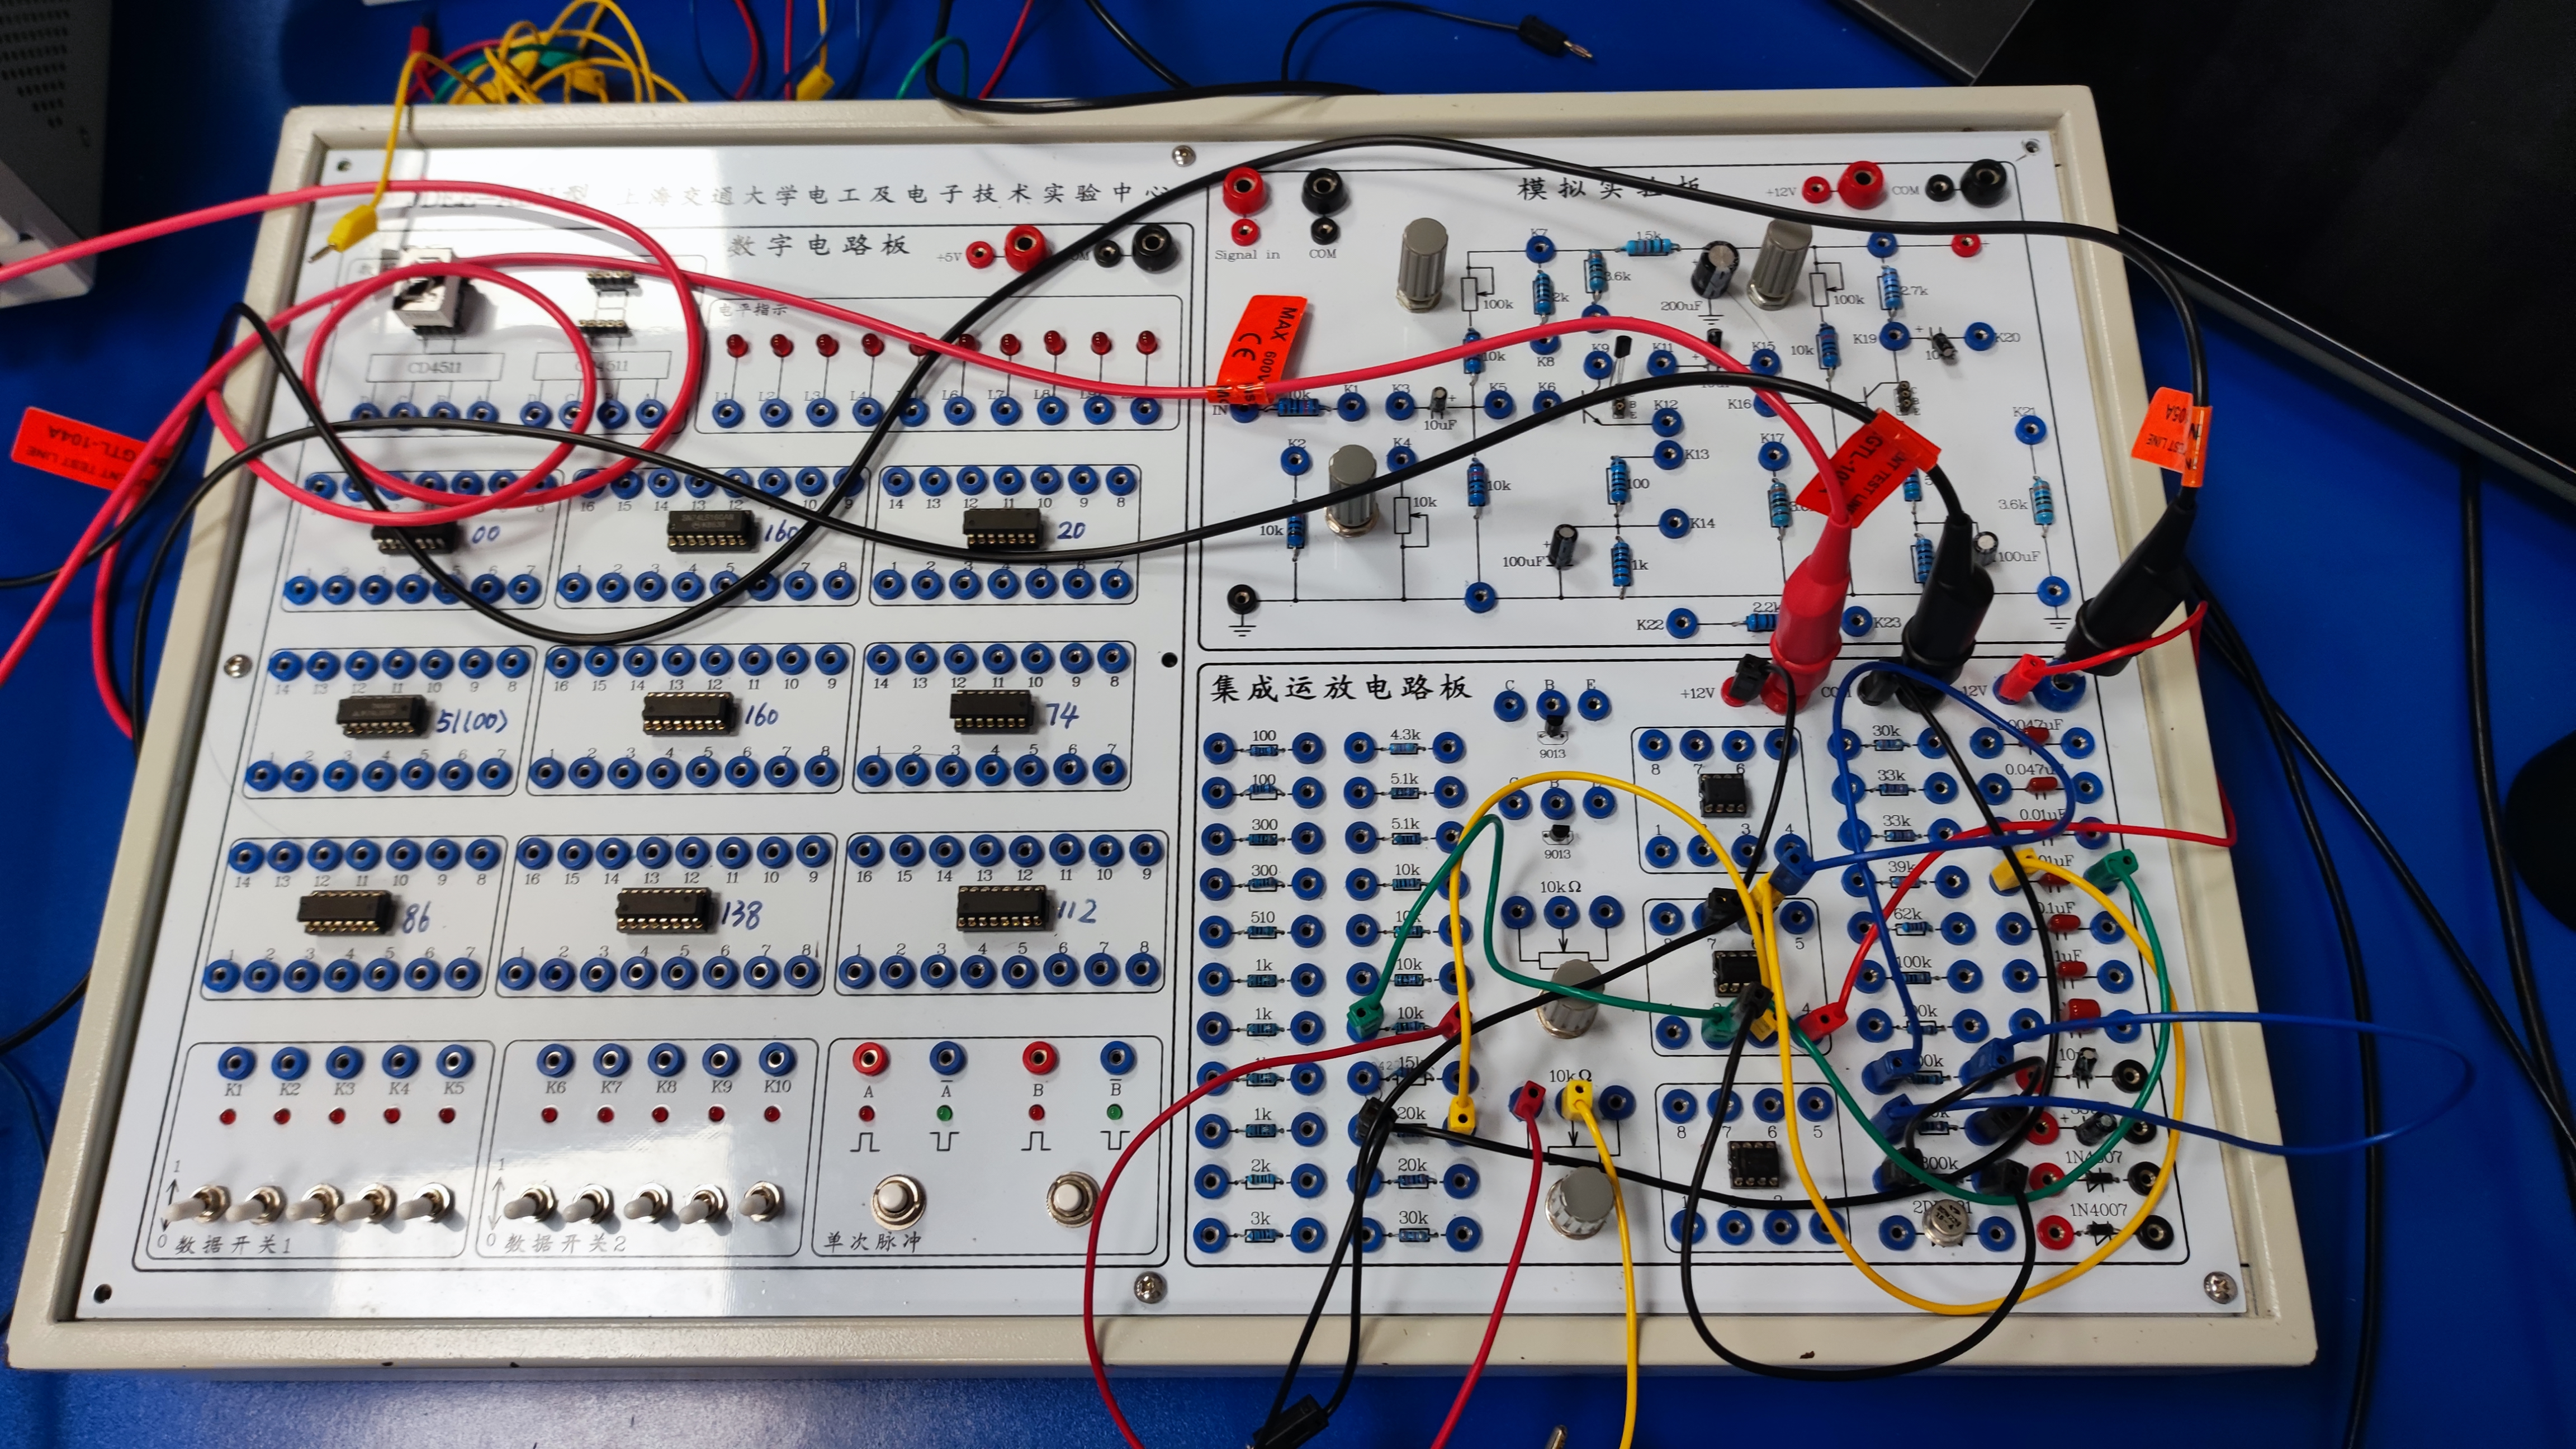
\includegraphics[width=0.9\linewidth]{../图片/积分器连线}
			\caption{积分器实物图}
		\end{minipage}		
	\end{figure}

	列写电路方程为
	$$
	\frac{u_i}{R_i}=-\frac{d Q}{d t}=-C \frac{d u_o}{d t}
	$$
	积分可得
	$$
	u_o=-\frac{1}{R_1 C} \int u_i d t
	$$
	
	线路中, $R_f$(兆欧级大电阻)接入电路，用于稳定直流工作点. 实验时使用了$500k\Omega$
	
	输入使用1kHz的0.2Vpp方波信号, 表达式为
	$$	
	f(t)=\left\{ 
	\begin{aligned}
		&0.1,& kT&<t\leqslant kT+\frac{T}{2}\\
		-&0.1,& kT+\frac{T}{2}&<t\leqslant kT+T
	\end{aligned}
	\right., T=0.001
	$$
	
	与同学交流发现常见的错误是使用$R_1C=0.5$的参数实验, 得到结果三角波信号幅度远大于400mVpp. 计算得到积分后的三角波Vpp为$\frac{1}{R_1\cdot C}\cdot 0.1\cdot \frac{T}{2}$, 故欲使得三角波Vpp为0.4Vpp, 应有$\frac{1}{R_1\cdot C}=2k\Omega\cdot F$. 使用电容大小为$0.01\mu F$, 使用滑动变阻器调节电阻至电阻大小为$40k\Omega$左右时, 发现恰好符合实验要求, 可见当有$R_f$时, 并不能完全理想的符合理论公式. 
	
	实验效果如图. 输出为输入方波的反相比例积分图像. 
	
	\begin{figure}[h]
		\begin{minipage}[t]{0.5\linewidth}
			\centering
			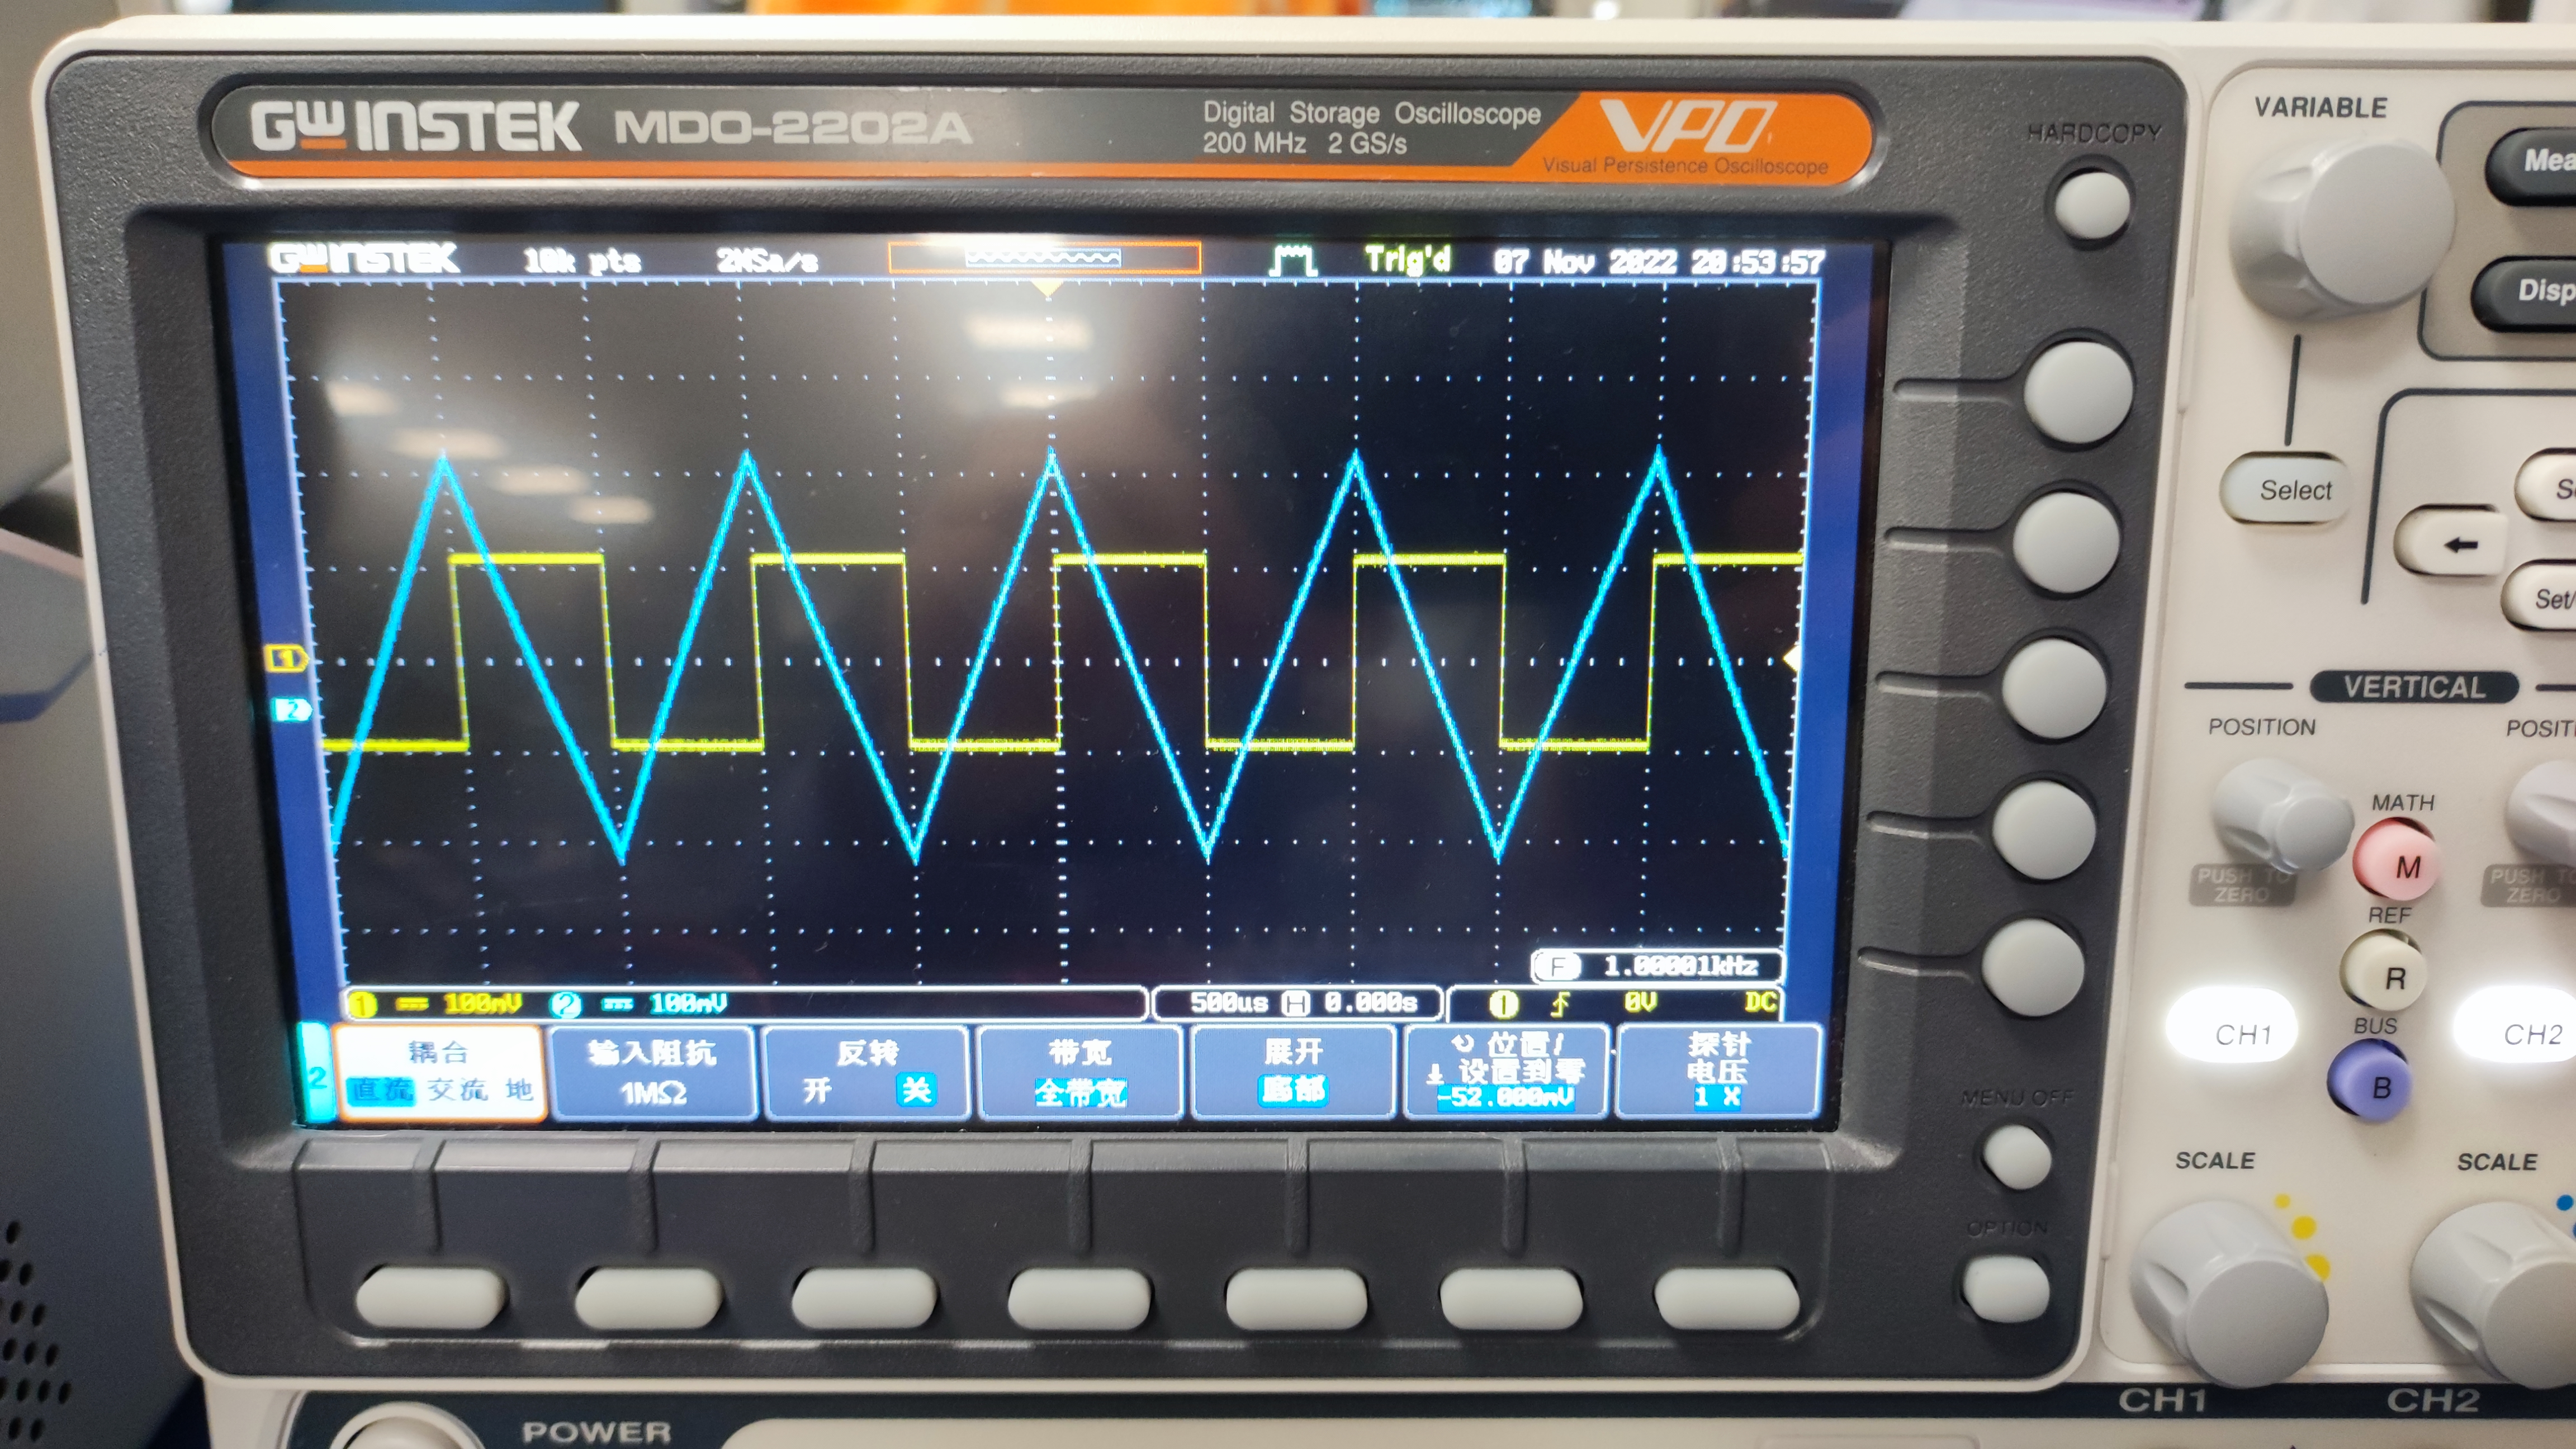
\includegraphics[width=0.9\linewidth]{../图片/积分器输入输出}
			\caption{积分器输入输出}
		\end{minipage}
		\begin{minipage}[t]{0.5\linewidth}
			\centering
			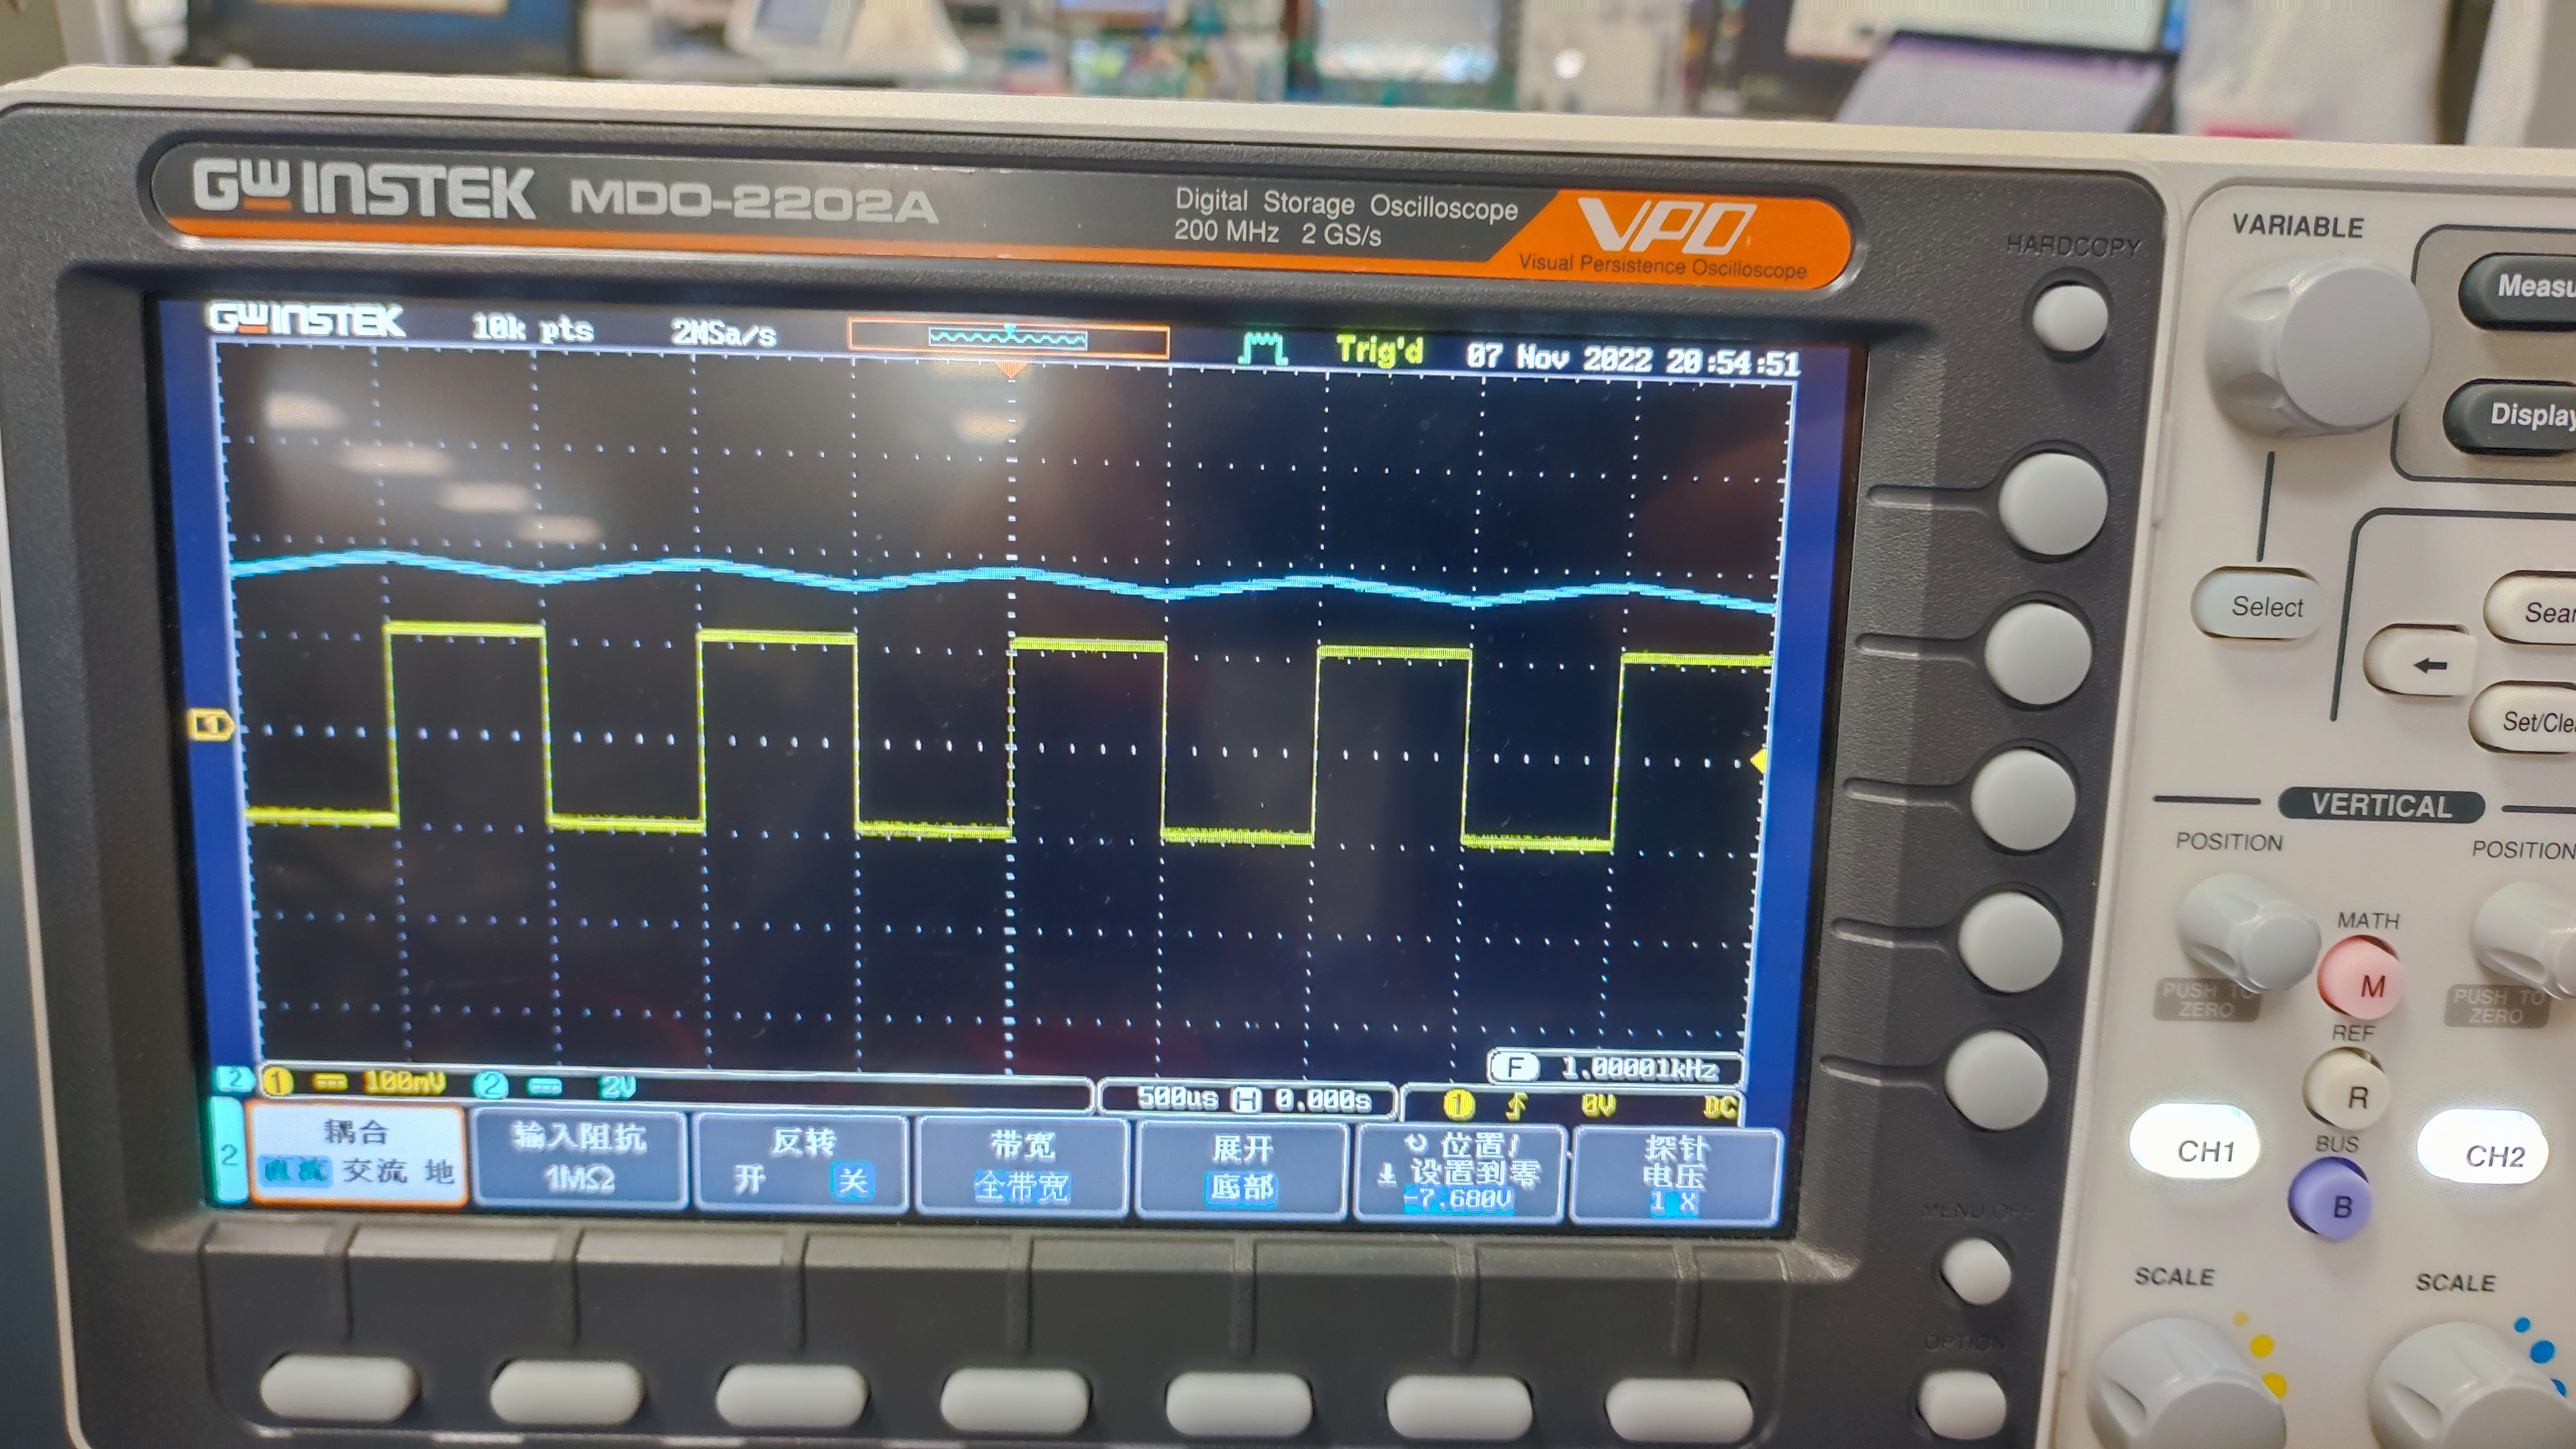
\includegraphics[width=0.9\linewidth]{../图片/积分器去掉r}
			\caption{积分器去除$R_f$}
		\end{minipage}		
	\end{figure}

	去除电路中的$R_f$, 此时测量的三角波信号Vpp更接近于积分理论推导结果, 但信号发生明显的偏置, 示波器上的图像向上偏移, 如图所示. 
	
	\subsection{微分器}
	如图所示, 连接微分器线路. 
	
	\begin{figure}[h]
		\begin{minipage}[t]{0.5\linewidth}
			\centering
			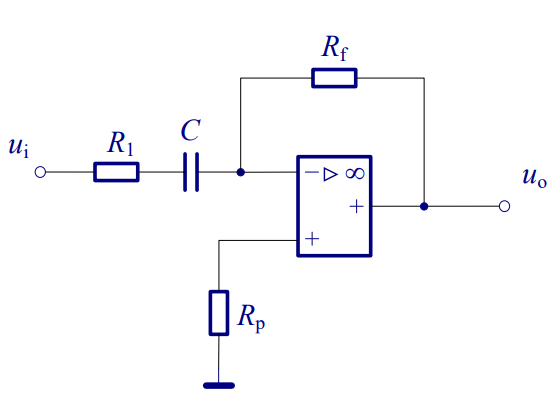
\includegraphics[width=0.6\linewidth]{微分器原理}
			\caption{微分器原理图}
		\end{minipage}
		\begin{minipage}[t]{0.5\linewidth}
			\centering
			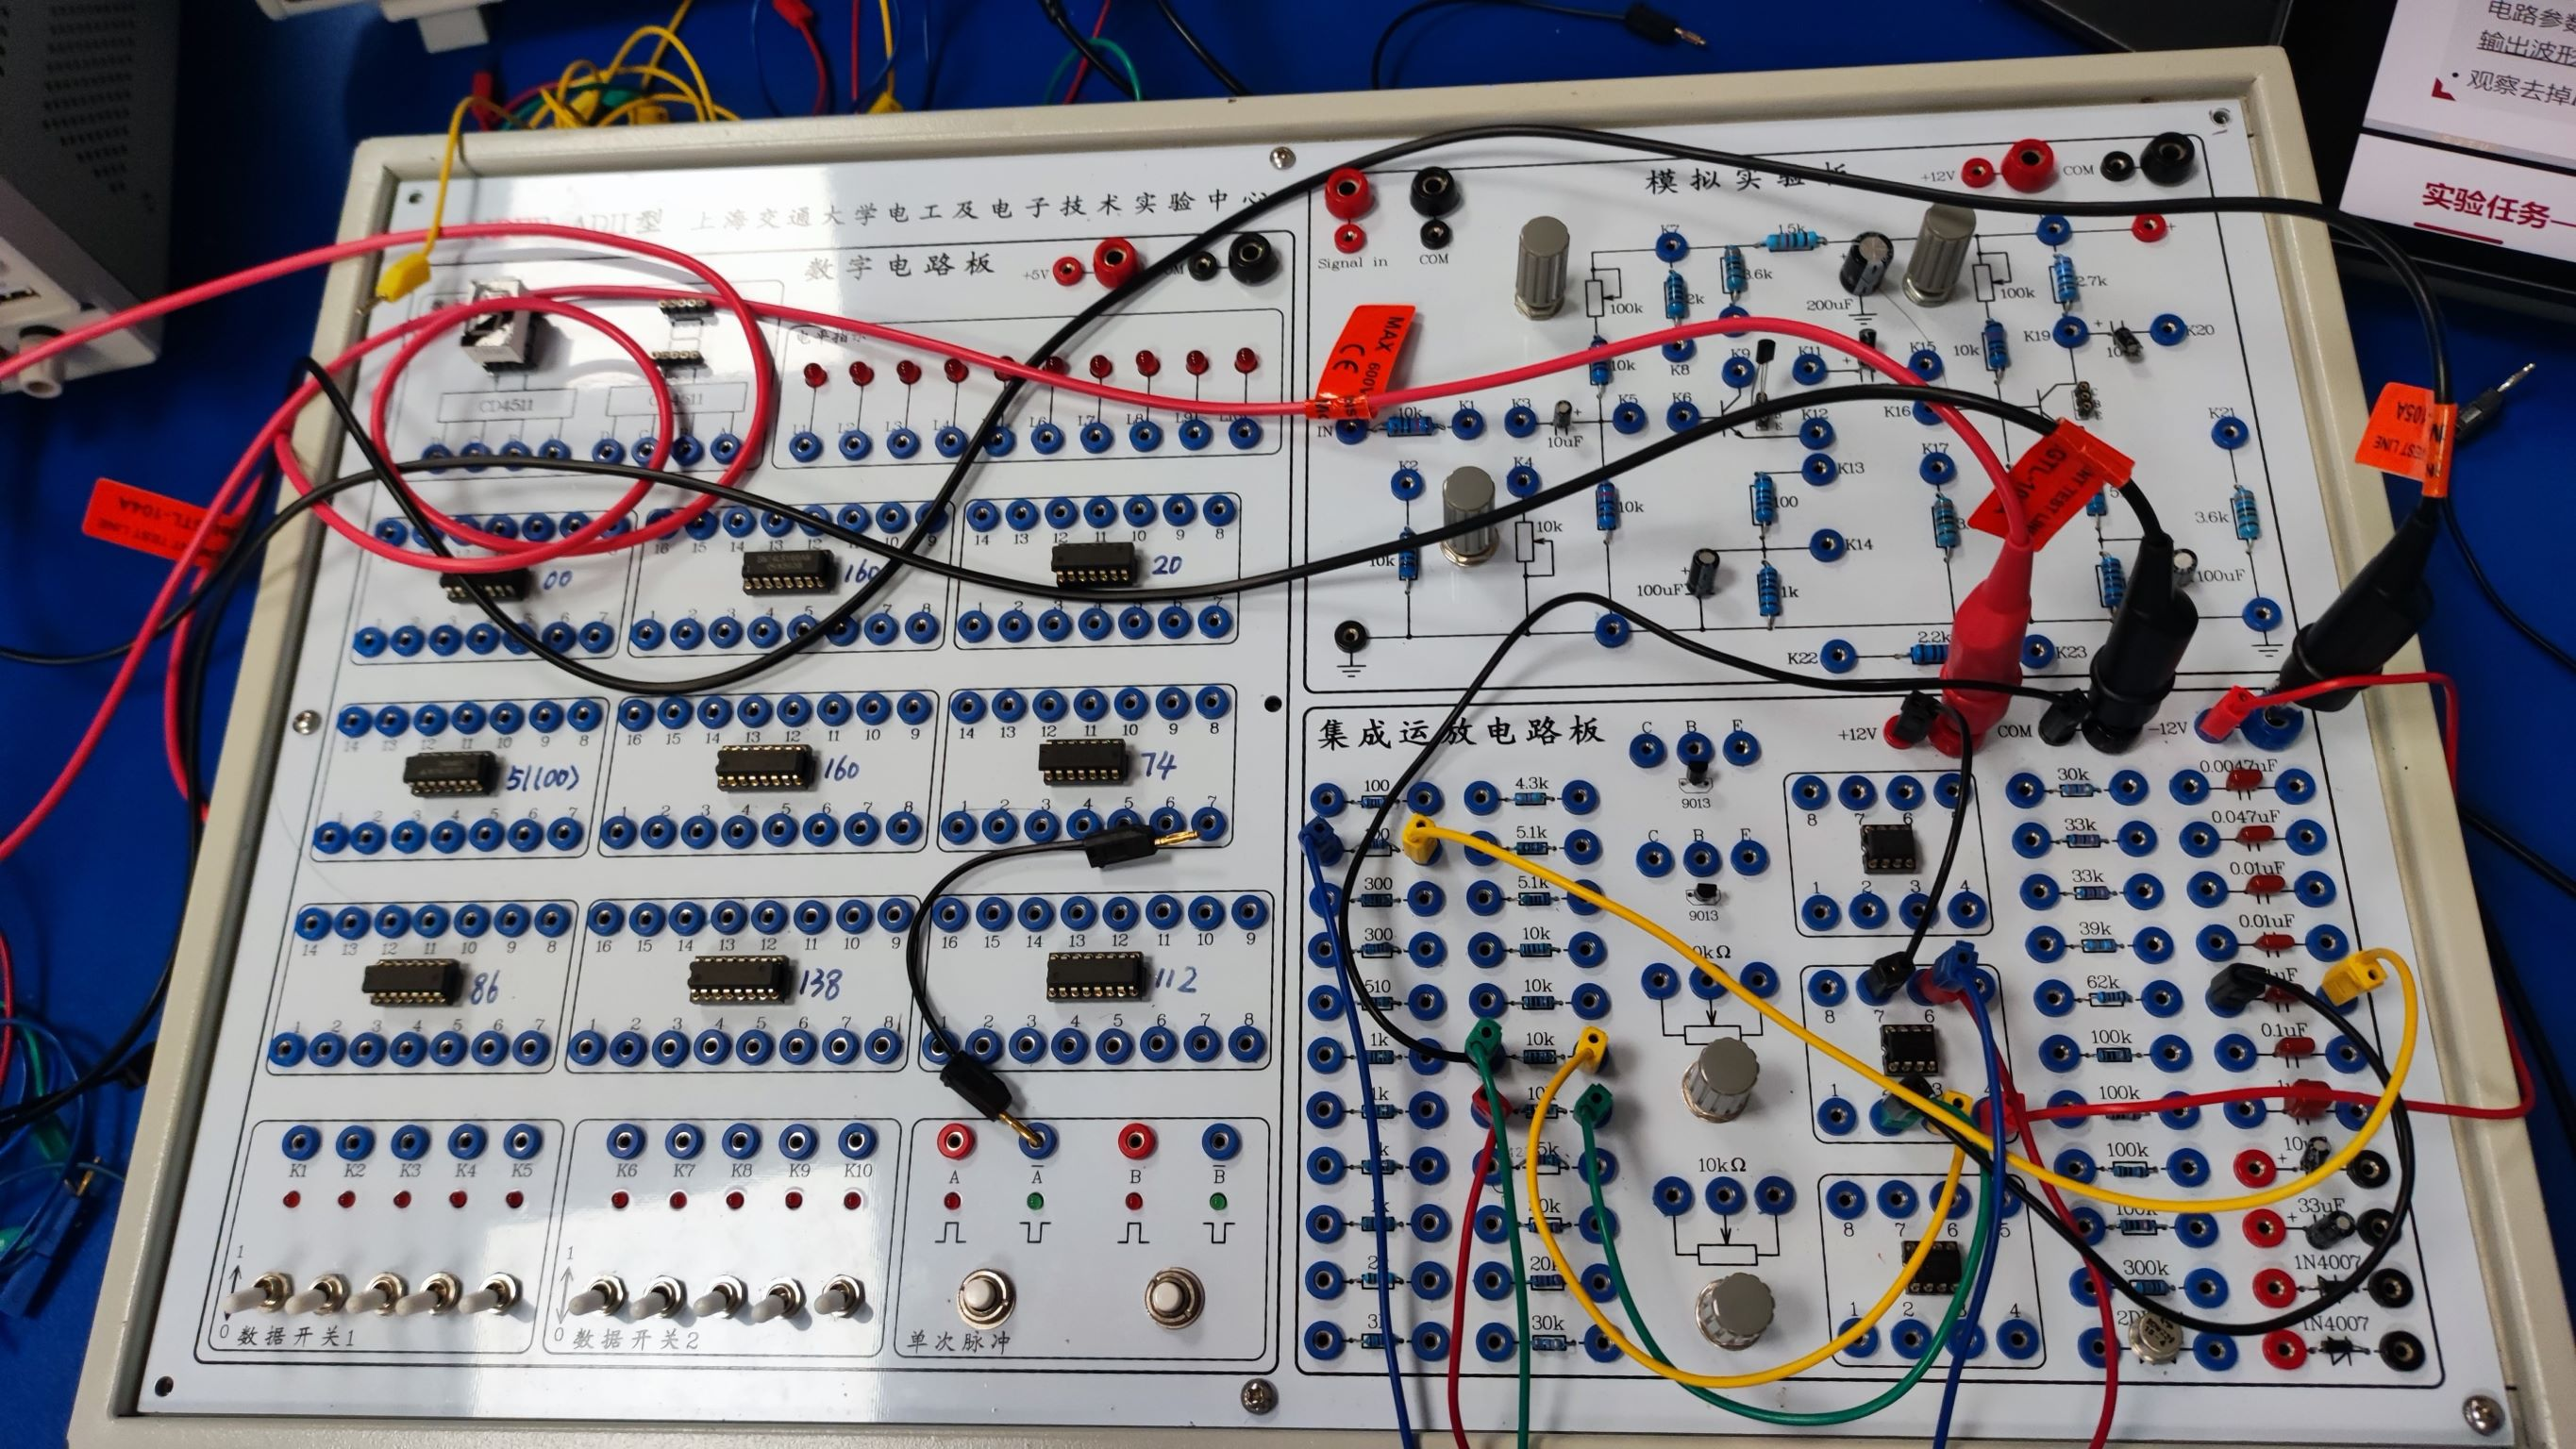
\includegraphics[width=0.9\linewidth]{../图片/微分器连线}
			\caption{微分器实物图}
		\end{minipage}		
	\end{figure}
	
	列写电路方程, 
	
	$$
	\left\{ 
	\begin{aligned}
		u_i&=i_1 R_1+u_c \\
		u_o&=i_o R_f \\
		i_1&+i_o=0
	\end{aligned}
	\right. 
	$$
	解得
	$$
	u_o=-R_f C \frac{d u_i}{d t}
	$$
	
	根据此式计算电路参数, 输入为200mVpp的三角波信号, 表达式为
	
	$$	
	f(t)=\left\{ 
	\begin{aligned}
		&0.1(t-kT),& kT&<t\leqslant kT+\frac{T}{2}\\
		-&0.1(t-kT-T),& kT+\frac{T}{2}&<t\leqslant kT+T
	\end{aligned}
	\right., T=0.001
	$$
	
	于是方波对应的Vpp大小为$2\cdot\frac{0.2}{0.5T}\cdot R_fC$, 要使方波幅值为800mVpp, 有$R_fC=0.001$. 使用电容大小为$0.1\mu F$, 电阻大小为$10k\Omega$, 起始时, 使用$R_1$大小为$100\Omega$. 示波器图像如第一张图所示. 加大$R_1$为$1k\Omega$, 图像变为第二张图所示. 可见$R_1$具有稳定的作用, 但过大时积分图像发生轻微失真. 
	\begin{figure}[h]
		\begin{minipage}[t]{0.5\linewidth}
			\centering
			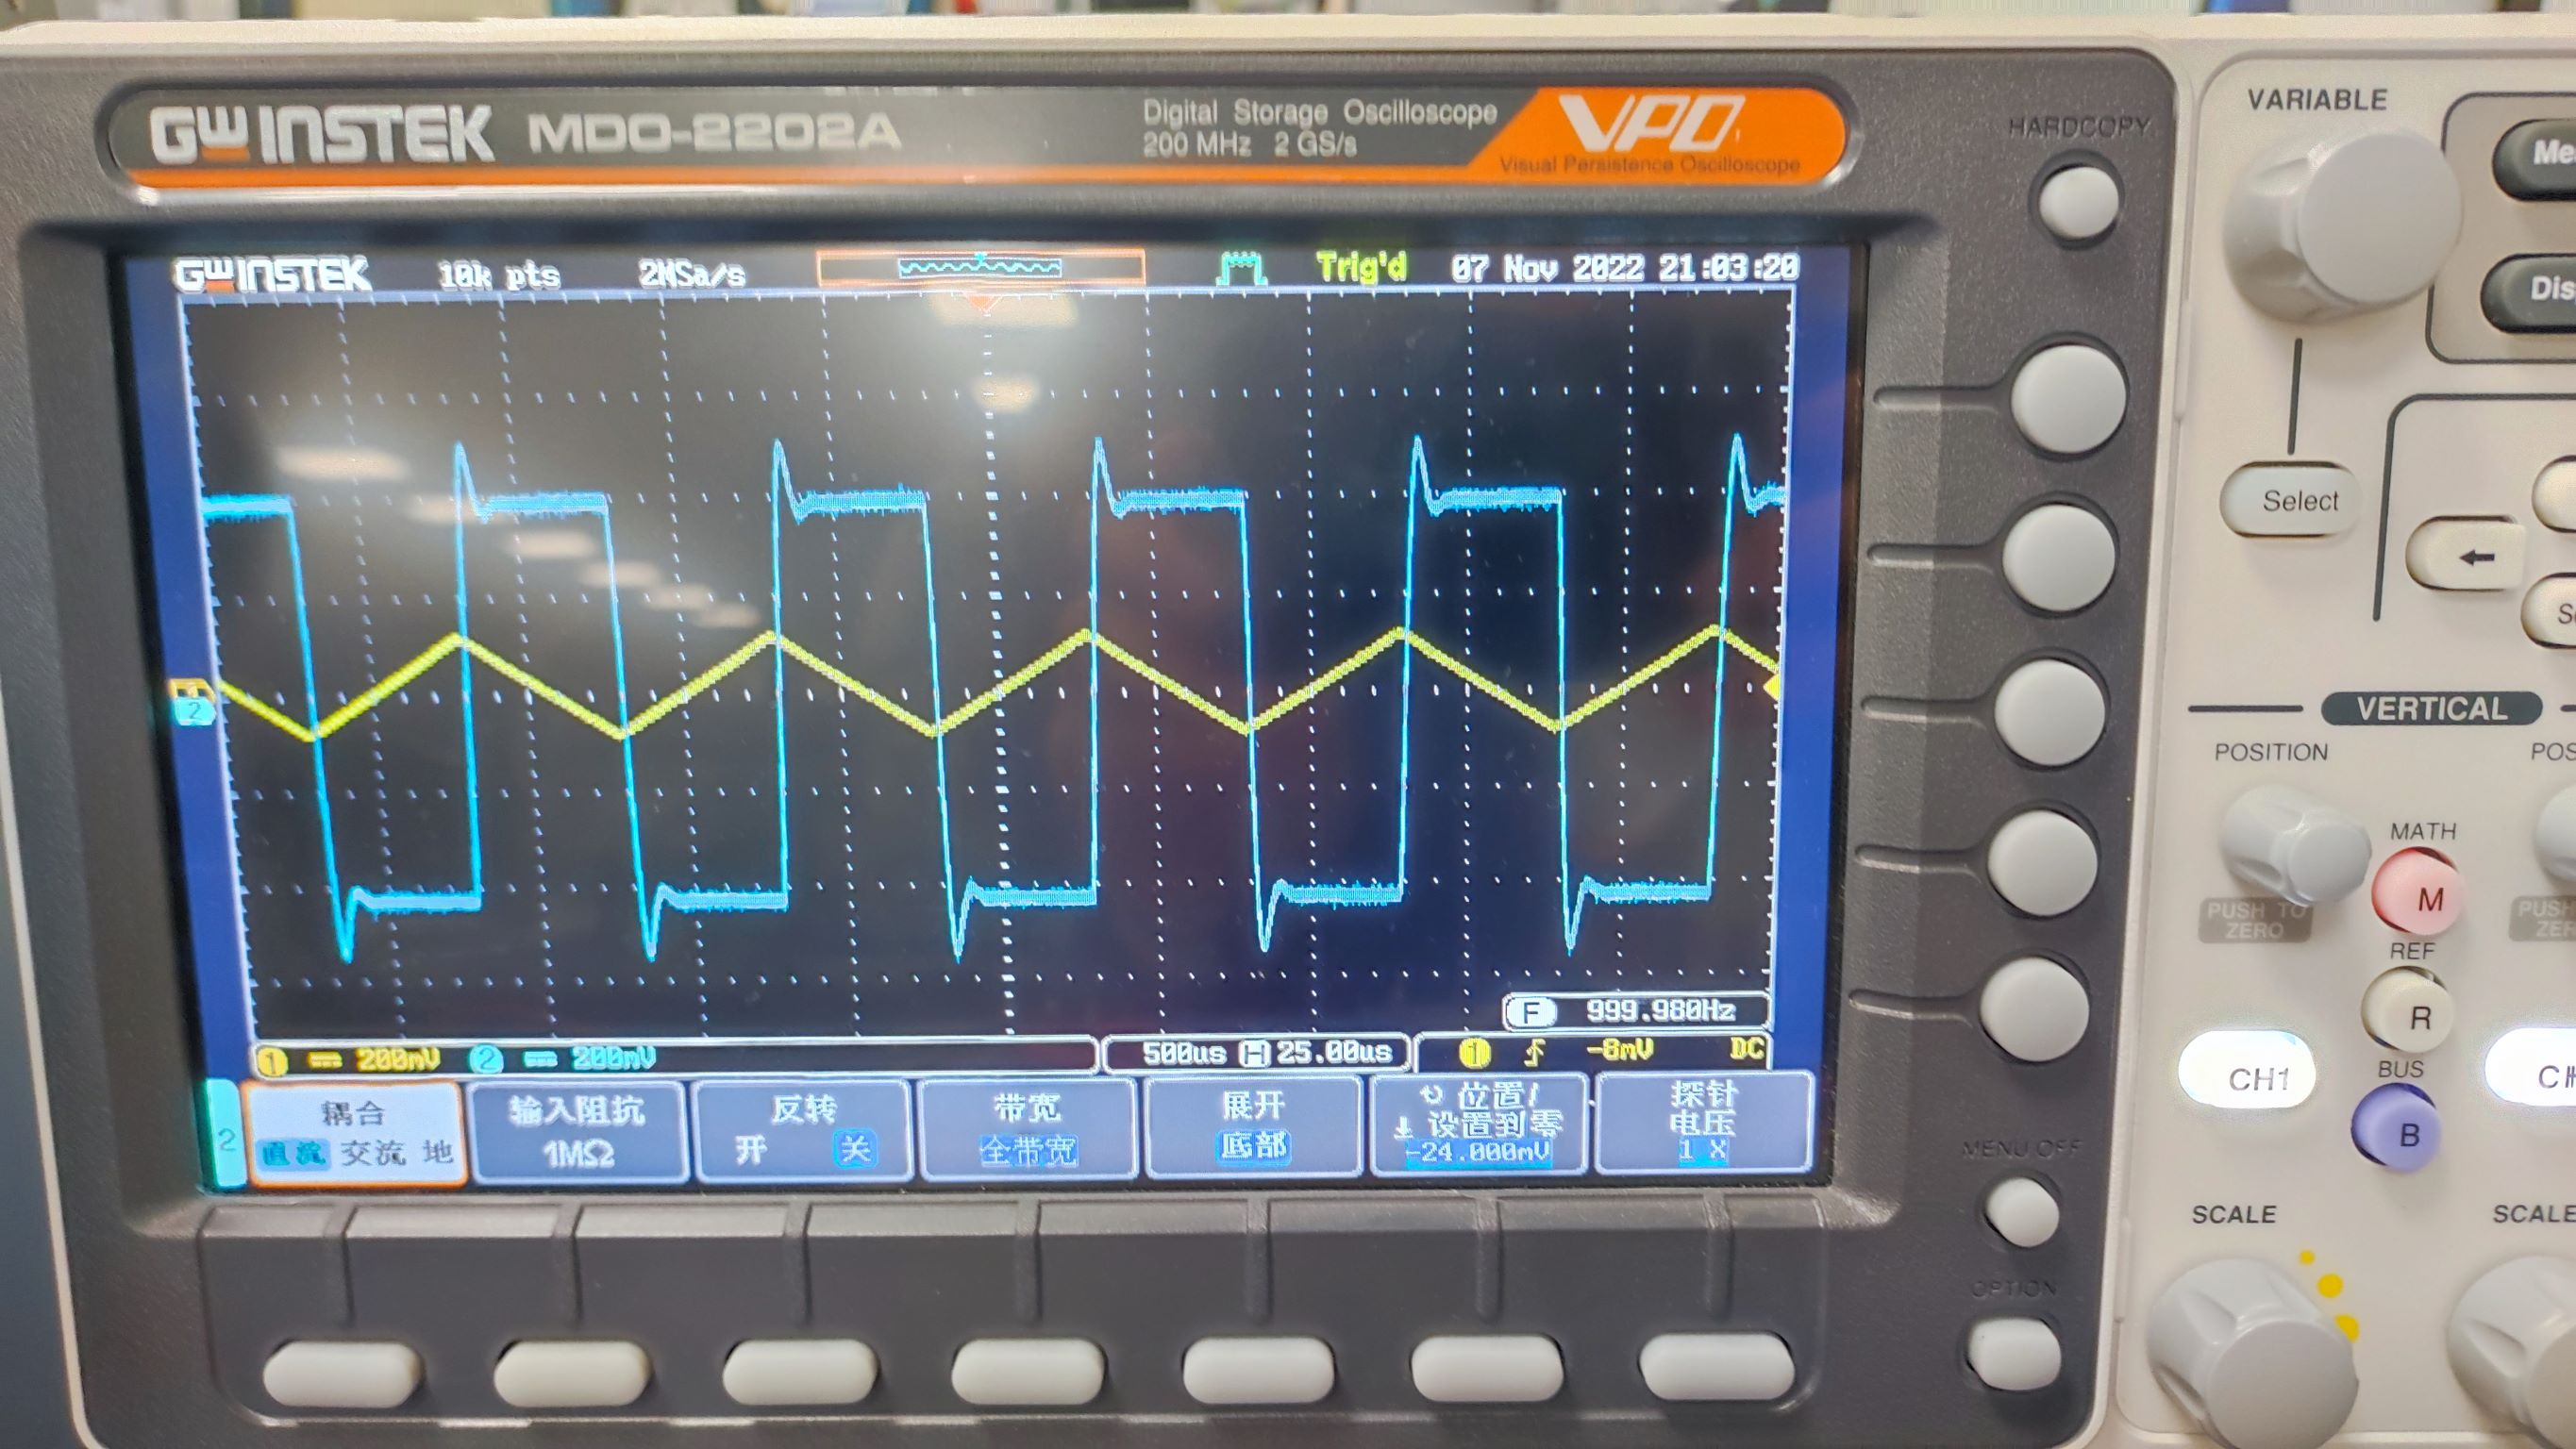
\includegraphics[width=0.9\linewidth]{../图片/微分器普通}
			\caption{微分输入输出}
		\end{minipage}
		\begin{minipage}[t]{0.5\linewidth}
			\centering
			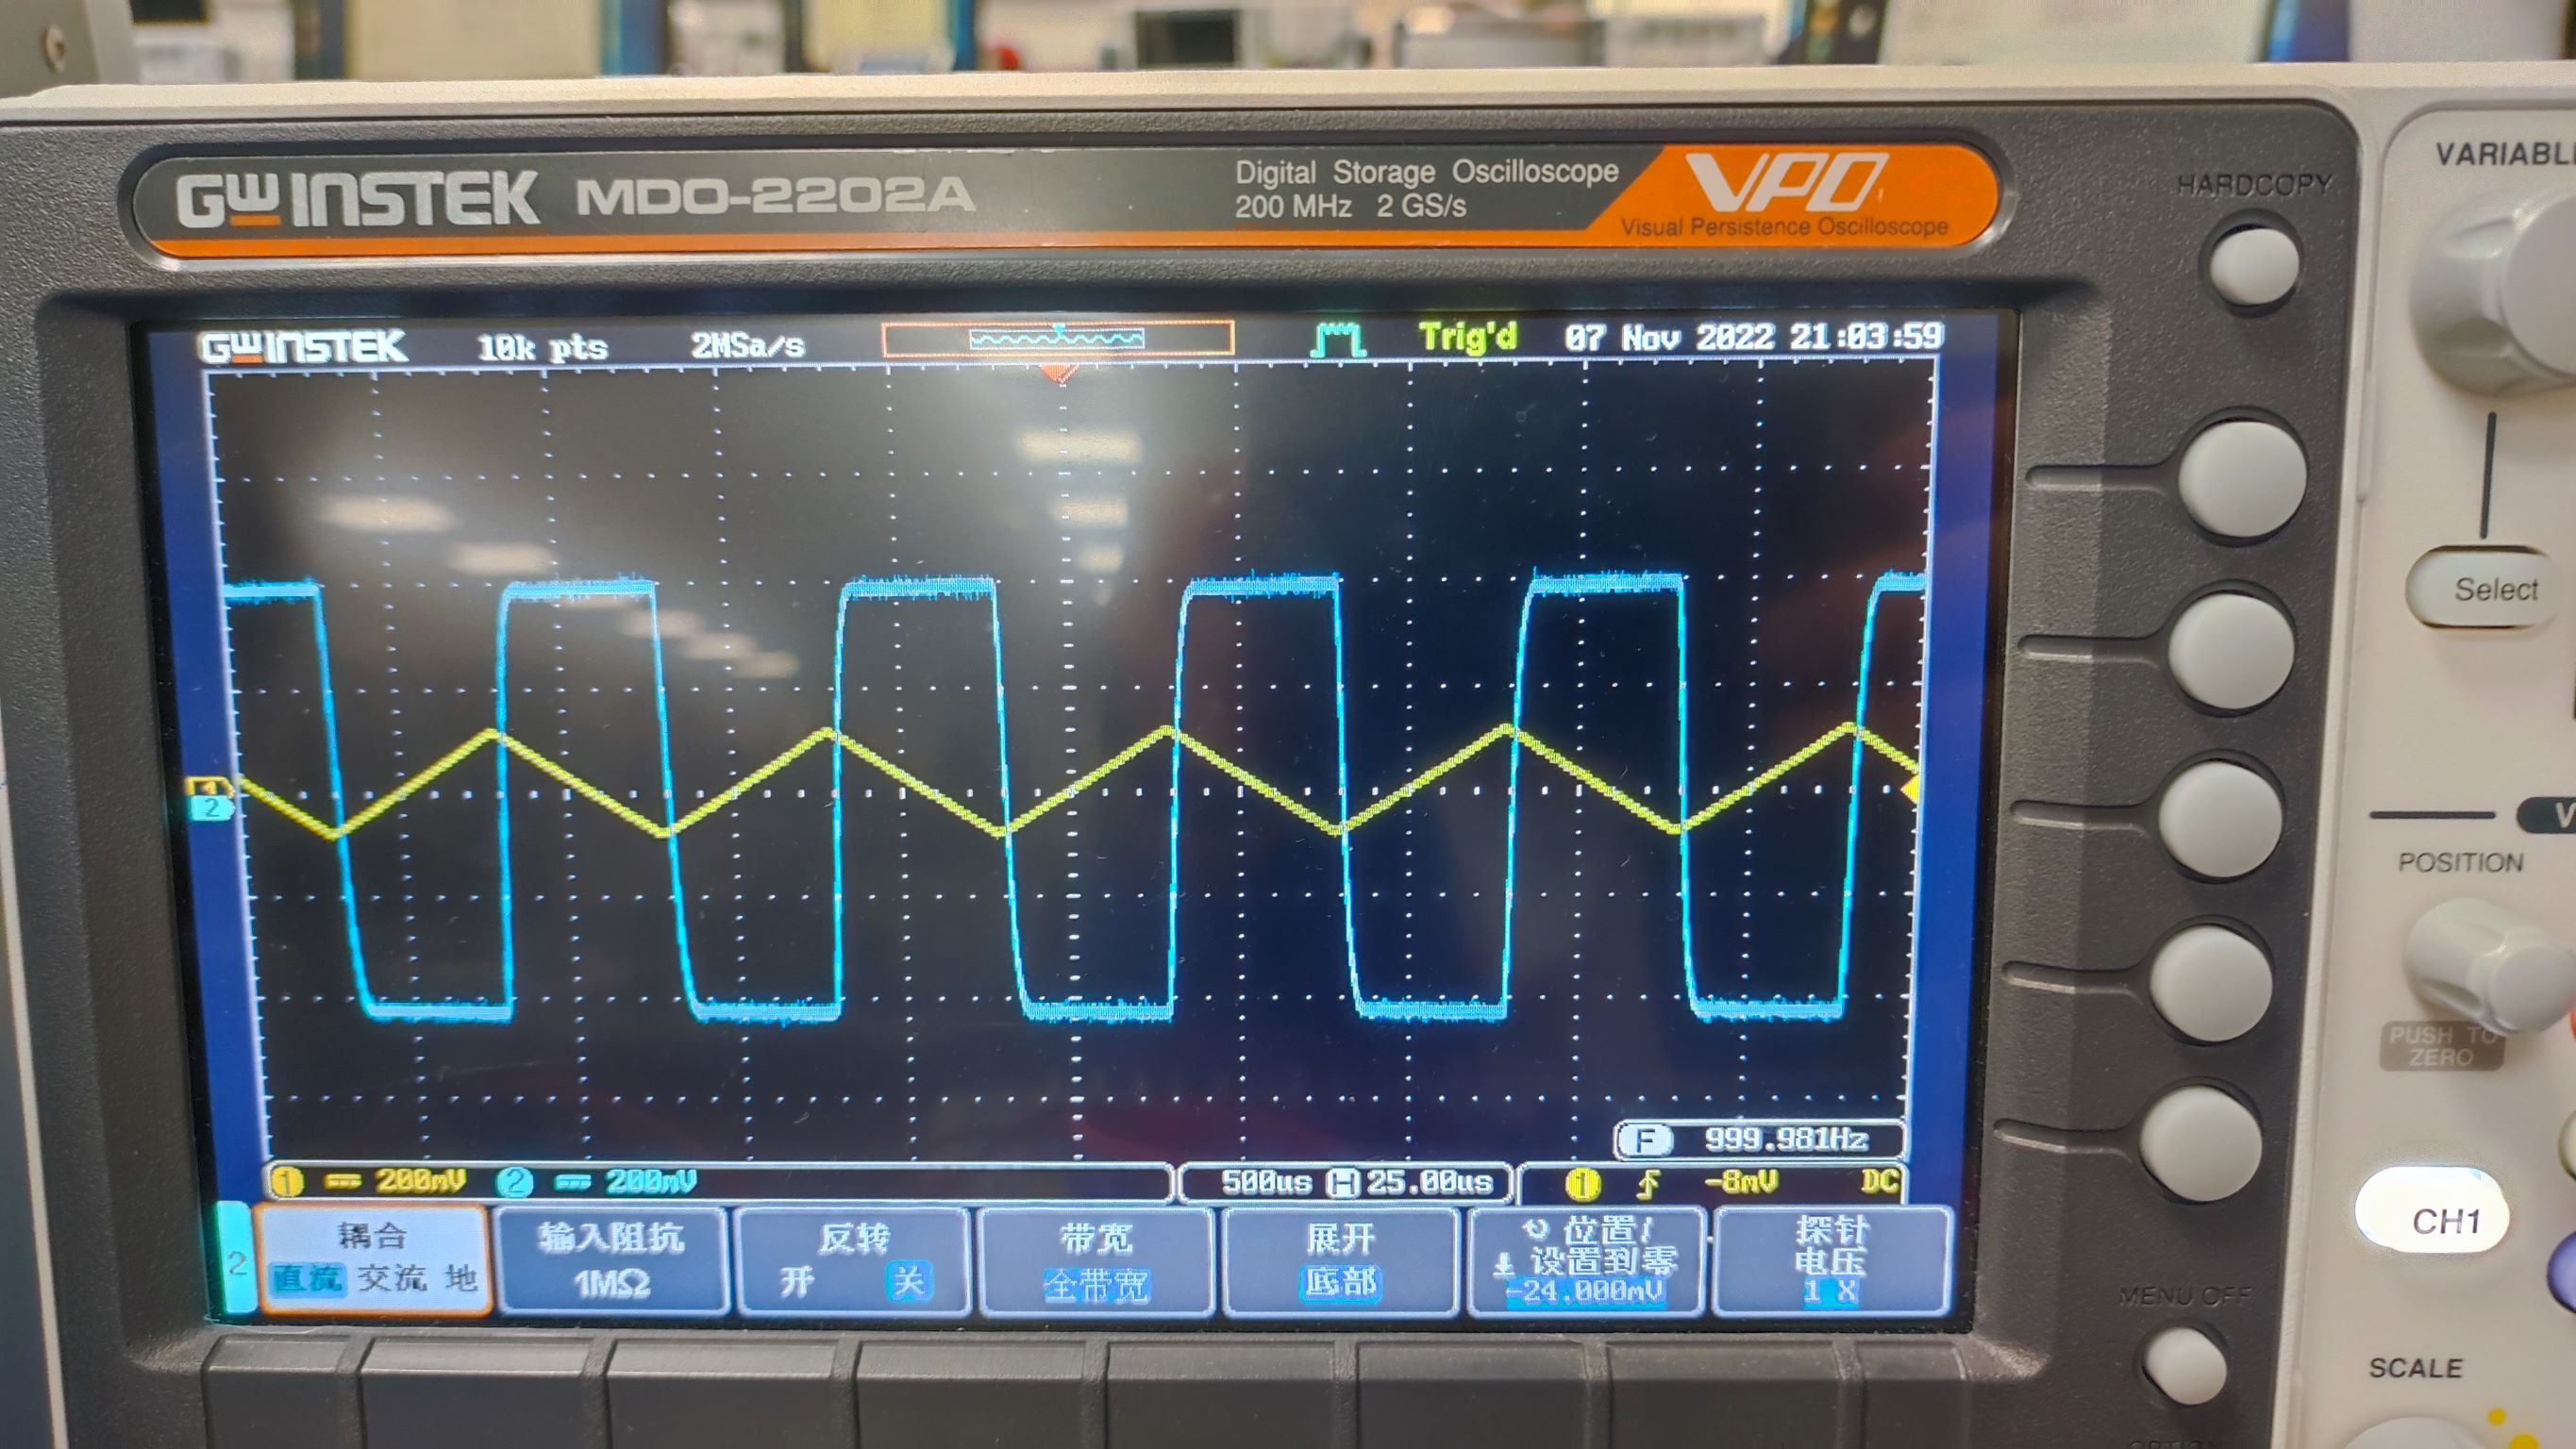
\includegraphics[width=0.9\linewidth]{../图片/微分器加大r}
			\caption{微分器加大$R_1$}
		\end{minipage}		
	\end{figure}

	去掉$R_1$, 图像如图所示, 震荡分量明显增大了. 

	\begin{figure}[h]
		\centering
		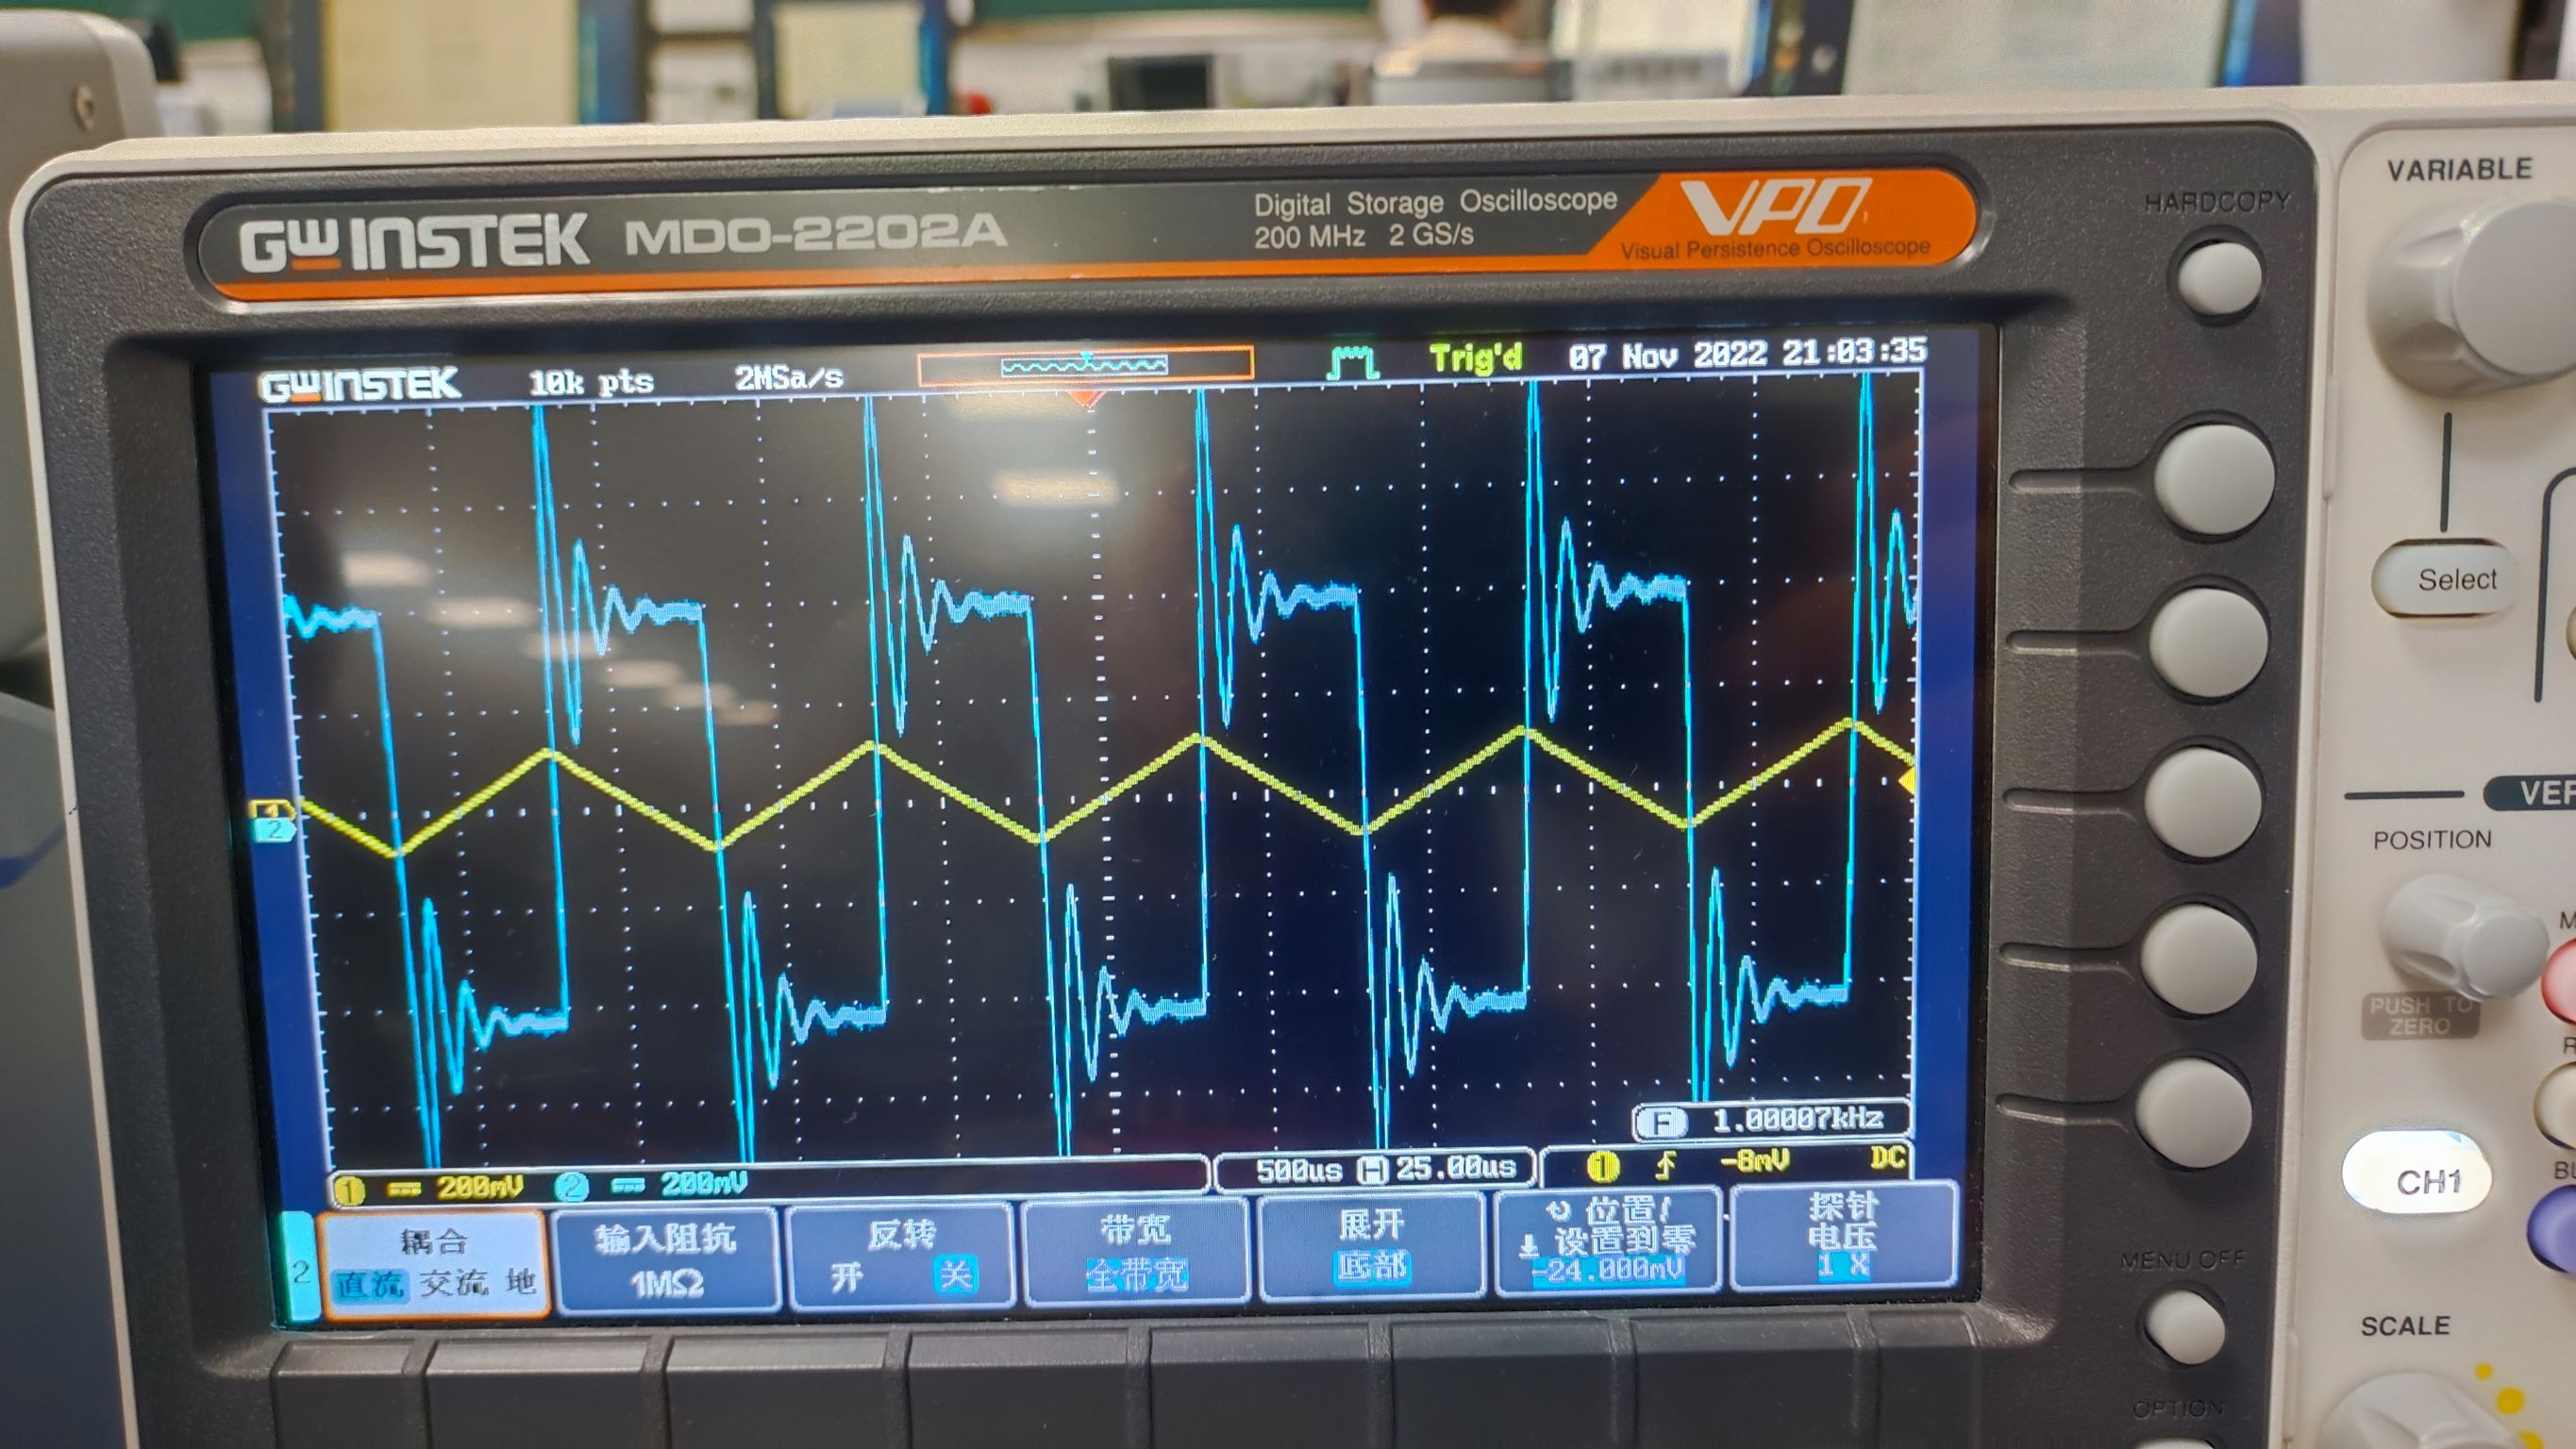
\includegraphics[width=0.5\linewidth]{../图片/微分器去掉r}
		\caption{微分器去掉$R_1$}
	\end{figure}
\section{模拟电路}
	先前模拟电路如图所示.
	\begin{figure}[h]
		\centering
		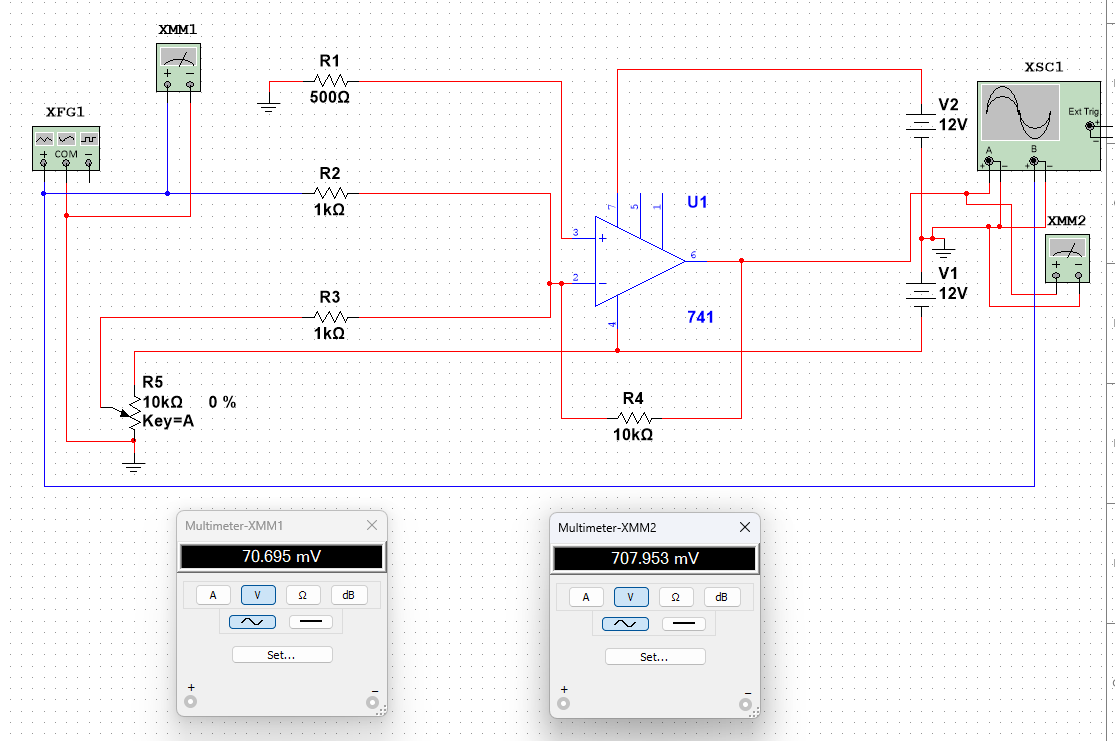
\includegraphics[width=0.5\linewidth]{../图片/加法器模拟}
		\caption{加法器模拟}
	\end{figure}
	\begin{figure}[h]
		\centering
		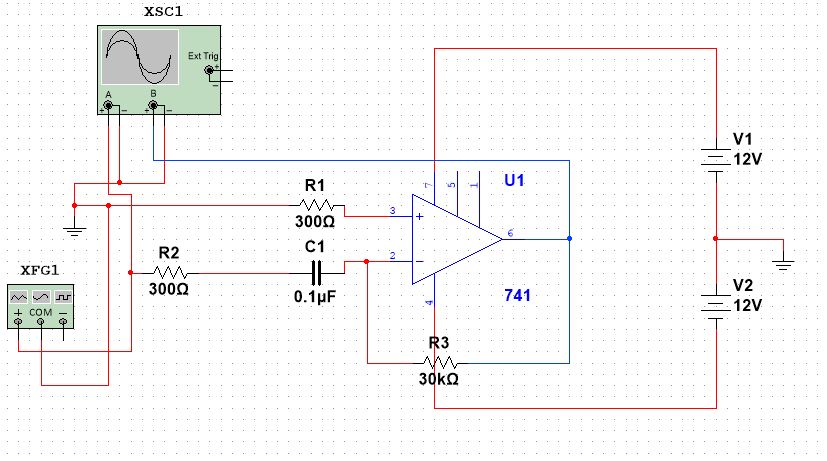
\includegraphics[width=0.5\linewidth]{../图片/微分器模拟}
		\caption{微分器模拟}
	\end{figure}
	\begin{figure}[h]
		\centering
		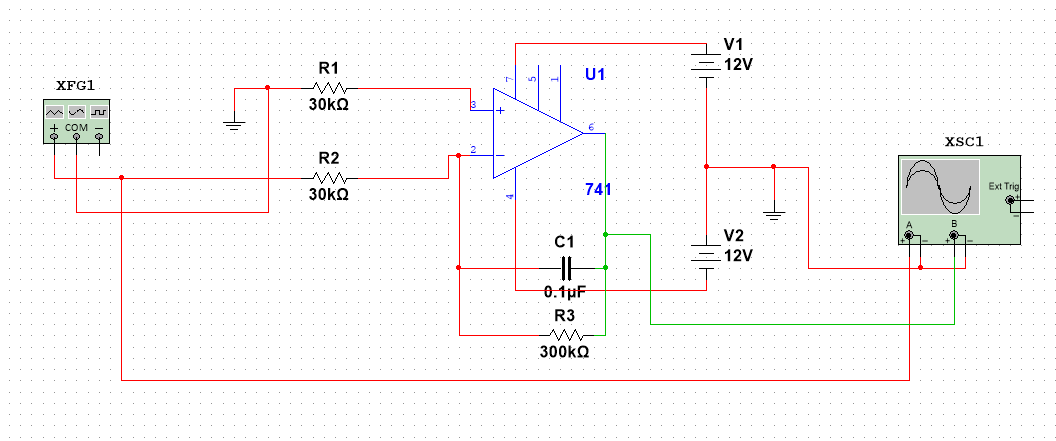
\includegraphics[width=0.5\linewidth]{../图片/积分器模拟}
		\caption{积分器模拟}
	\end{figure}
\end{document}